\chapter{The inverse ray mapping method: analytic approach}\label{chap:raymapping1}
PS ray tracing based on the source and the target PS constitutes an improvement of MC and QMC ray tracing. 
Now, a method that employs not only the source and the target PS but also the PS of \textit{all} the other lines that constitute the optical system is introduced. %Furthermore, instead of starting from the source, the new approach is an inverse method which starts considering rays on target PS.
All lines can be modeled as detectors of the incident light and emitters of the reflected light.
Moreover, we assume that the source can only emit light and the target can only receive light.
Therefore, one PS is taken into account for the source and one for the target while both the source and target phase spaces are considered for the other lines. Every line of the system (except for the source \point{S} and the target \point{T}) constitutes
the target for incident rays and the source for reflected rays. Therefore, two different phase spaces are considered for the reflectors and one PS for
\point{S} and \point{T}. All these phase spaces are connected through a map which relates the rays coordinates on every PS. In order to compute the target photometric variables an inverse ray mapping reconstruction from the target to the source is involved.
\\\indent
In this chapter two different optical systems are investigated.
First, the method is explained for the two-faceted cup. 
Then, it is extended to a more complicated system, the so-called multi-faceted cup, which is formed by only straight lines segments.
\section{Explanation of the method}
Using the PS of \textit{all} the lines that form the system, a map from the source to the target of the system is constructed. This map can be written as the concatenation of many maps which
can be classified as two different kinds of maps, i.e. the map that connects the source and the target PS of two \textit{different} lines and the map that connects the target and the source PS of the \textit{same} line.
Employing the inverses of these maps we are able to detect the parts on target PS illuminated by the source.
All the PS considered are divided into regions, the boundaries of which can be determined exactly for systems formed by straight lines.
We make the assumption of a Lambertian source; hence, the luminance is a positive constant when different from $0$. 
As a consequence, the output intensity along a given direction is given by the total width of all the patches with positive luminance, measured along that direction.\\ \indent Next, the details of the procedure are explained for a very simple optical system: the two-faceted-cup.
\section{The two-faceted cup}
A two-faceted cup is formed by a source \point{S}, a target \point{T} and two reflectors which are straight lines segments. 
As an example, we consider the two-faceted cup introduced in Chapter \ref{chap:raytracing} and depicted in Figure \ref{fig:cup}.
We use the same notations of Chapter \ref{chap:PS} to indicate the PS $\mbox{\set{S}{}{}}=\mbox{\set{Q}{}{}}\times\mbox{\set{P}{}{}}$ and the rays coordinates 
$(\variabile{q}, \variabile{p})$ in \set{S}{}{}.\\ \indent
Let's now introduce some new notation. 
The source and the target PS of a line $\lineai$ are indicated with \set{S}{\lineai}{} and \set{T}{\lineai}{}, respectively.
The coordinates of every ray that reaches the line $\lineai\in\{1, 2, 3\}$ are indicated  with $(\pos{t,}{\lineai}, \dir{t,}{\lineai})$ on \set{T}{\lineai}{}.
After reflection, the ray leaves line $\lineai \in\{1, 2, 3\}$ at the same position and with a new direction, the new coordinates are indicated with 
$(\pos{s,}{\lineai}, \dir{s,}{\lineai})$ on \set{S}{\lineai}{}.
Note that $\pos{s,}{\lineai}= \pos{t,}{\lineai}$ while $\dir{s,}{\lineai}$ is obtained applying the reflection law to the direction coordinate $\dir{t,}{\lineai}$ of the incident ray.
The phase spaces \set{S}{\lineai}{} and  \set{T}{\lineai}{} of each line $\lineai$ are partitioned into different regions, (\set{S}{\lineai,}{\lineaj})$_{\lineaj=2, 3, 4}$ and (\set{T}{\lineai,}{\lineak})$_{\lineak=1, 2, 3}$, respectively, where $\lineaj\neq \lineai$ is the index of the line that is illuminated by $\lineai$ and $\lineak\neq\lineai$ is the index of the line that illuminates $\lineai$. Hence, we indicate with \set{S}{\lineai,}{\lineaj}$\subset$ \set{S}{\lineai}{} the part of \set{S}{\lineai}{} corresponding to rays that illuminate line $\lineaj$ and with \set{T}{\lineai,}{\lineak} $\subset$ \set{T}{\lineai}{} the part of \set{T}{\lineai}{} corresponding to rays originating from the line $\lineak$. Note that, due to the fact that the source only emits light, we do not define its target phase space \set{T}{$1$}{}. Similarly, since the target only receives light, its source phase space \set{S}{$4$}{} is not defined.
For the two-faceted cup, six different phase spaces need to be considered which are given by the following expressions:
\begin{equation}
\label{SPS}
\begin{split}
 \mbox{\set{S}{$1$}{}} & = \mbox{\set{S}{$1$,}{$2$}}\cup
 \mbox{\set{S}{$1$,}{$3$}} \cup \mbox{\set{S}{$1$,}{$4$}},\\
\mbox{\set{S}{$2$}{}} & =  \mbox{\set{S}{$2$,}{$3$}} \cup \mbox{\set{S}{$2$,}{$4$}},\\
\mbox{\set{S}{$3$}{}} & =  \mbox{\set{S}{$3$,}{$2$}} \cup \mbox{\set{S}{$3$,}{$4$}},\\
\mbox{\set{T}{$2$}{}} & = \mbox{\set{T}{$2$,}{$1$}} \cup \mbox{\set{T}{$2$,}{$3$}},\\
\mbox{\set{T}{$3$}{}} & = \mbox{\set{T}{$3$,}{$1$}}\cup \mbox{\set{T}{$3$,}{$2$}},\\
\mbox{\set{T}{$4$}{}} & = \mbox{\set{T}{$4$,}{$1$}}\cup \mbox{\set{T}{$4$,}{$2$}}\cup
\mbox{\set{T}{$4$,}{$3$}}.
\end{split}
 \end{equation}
We need to note that, as the source cannot receive light and the target cannot emit light,  the regions $(\mbox{\set{S}{\lineai,}{$1$}})_{\lineai=2,3}$ and $(\mbox{\set{T}{\lineai,}{$4$}})_{\lineai=2, 3}$ are not considered.
The boundaries $\partial \mbox{\set{S}{\lineai,}{\lineaj}}$ are mapped into the boundaries $\partial \mbox{\set{T}{\lineaj,}{\lineai}}$ for every $\lineai=\{1, 2, 3\}$ 
and $\lineaj=\{2, 3,4\}$ with $\lineaj\neq \lineai$ (edge-ray principle \cite{Ries}). For the two-faceted cup and for all systems that are formed by straight lines, they are determined analytically as explained in the following.
Given two lines $\lineai$ and $\lineak$
with $\lineai\neq \lineak$, we show how to compute the boundaries of the region formed by the rays that leave line $\lineai$ and hit line $\lineak$. We do that both on \set{S}{\lineai}{} and on \set{T}{\lineak}{}.
We indicate with $(\variable{x}_{\lineai, \ell}, \variable{z}_{\lineai, \ell})$ and with $(\variable{x}_{\lineai, \textrm{r}},\variable{z}_{\lineai, \textrm{r}})$ the coordinates of the points located at the left and the right extreme of line $\lineai$, respectively.
Similarly, $(\variable{x}_{\lineak, \ell}, \variable{z}_{\lineak, \ell})$ and $(\variable{x}_{\lineak, \textrm{r}},\variable{z}_{\lineak, \textrm{r}})$ are the coordinates of the points located at the left and the right extreme of line $\lineak$, respectively.
The boundaries $\partial$\set{S}{\lineai,}{\lineak} and $\partial$\set{T}{\lineak,}{\lineai} are obtained considering all the rays that leave the extremes of line $\lineai$ 
and all the rays that reach the extremes of the target.
Given two lines $\lineai$ and $\lineak$ with $\lineai\neq \lineak$, $\partial$\set{S}{\lineai,}{\lineak} and $\partial$\set{T}{\lineak,}{\lineai}
are formed by four different curves,
two of them are given by all the rays that leave the end points of line $\lineai$ and hit line $\lineak$ and, the others two are given by the rays
that leave the extremes of line $\lineai$ and hit the extremes of line $\lineak$.
The boundaries $\partial$\set{S}{\lineai,}{\lineak} and $\partial$\set{T}{\lineak,}{\lineai} are given by:
 \begin{equation}
\label{eq:analytic_boundaries}
 \begin{split}
 \partial\mbox{\set{S}{i,}{k}} & = \partial\mbox{\setbound{S}{i,}{k}{\,1}}\cup \partial\mbox{\setbound{S}{i,}{k}{\,2}} \cup \partial\mbox{\setbound{S}{i,}{k}{\,3}}\cup \partial\mbox{\setbound{S}{i,}{k}{\,4}},\\
\partial\mbox{\set{T}{k,}{i}} & = \partial\mbox{\setbound{T}{k,}{i}{\,1}}\cup \partial\mbox{\setbound{T}{k,}{i}{\,2}}\cup \partial\mbox{\setbound{T}{k,}{i}{\,3}}\cup \partial\mbox{\setbound{T}{k,}{i}{\,4}}.
 \end{split}
 \end{equation}
In the following we explain in more details the case of $\variabile{\lineai}=1$ and $\variabile{\lineak}=4$; see Fig. \ref{fig:cups}.
\begin{figure}[h]
\centering
\begin{subfigure}{.48\textwidth}
  \centering
  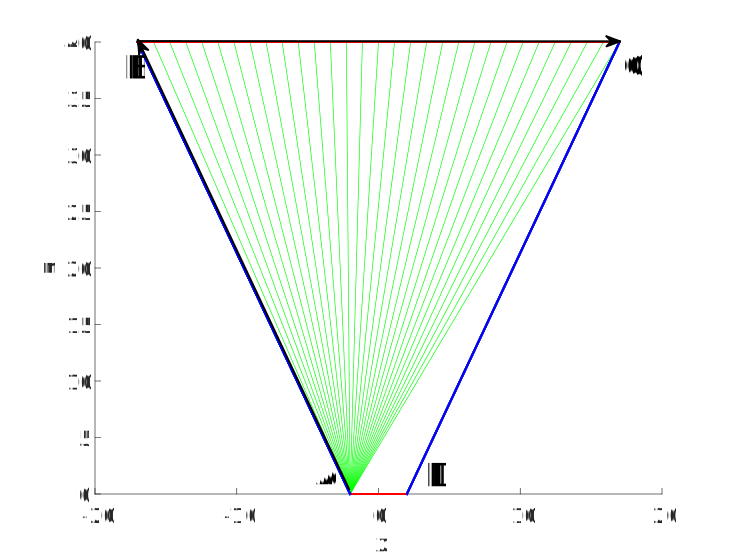
\includegraphics[width=\textwidth]{rays_cup1}
  \caption{Rays that leave the left end point of the source (line $1$) and trace out the target (line $4$).}
  \label{fig:cup1}
\end{subfigure}%
\begin{subfigure}{.48\textwidth}
  \centering
  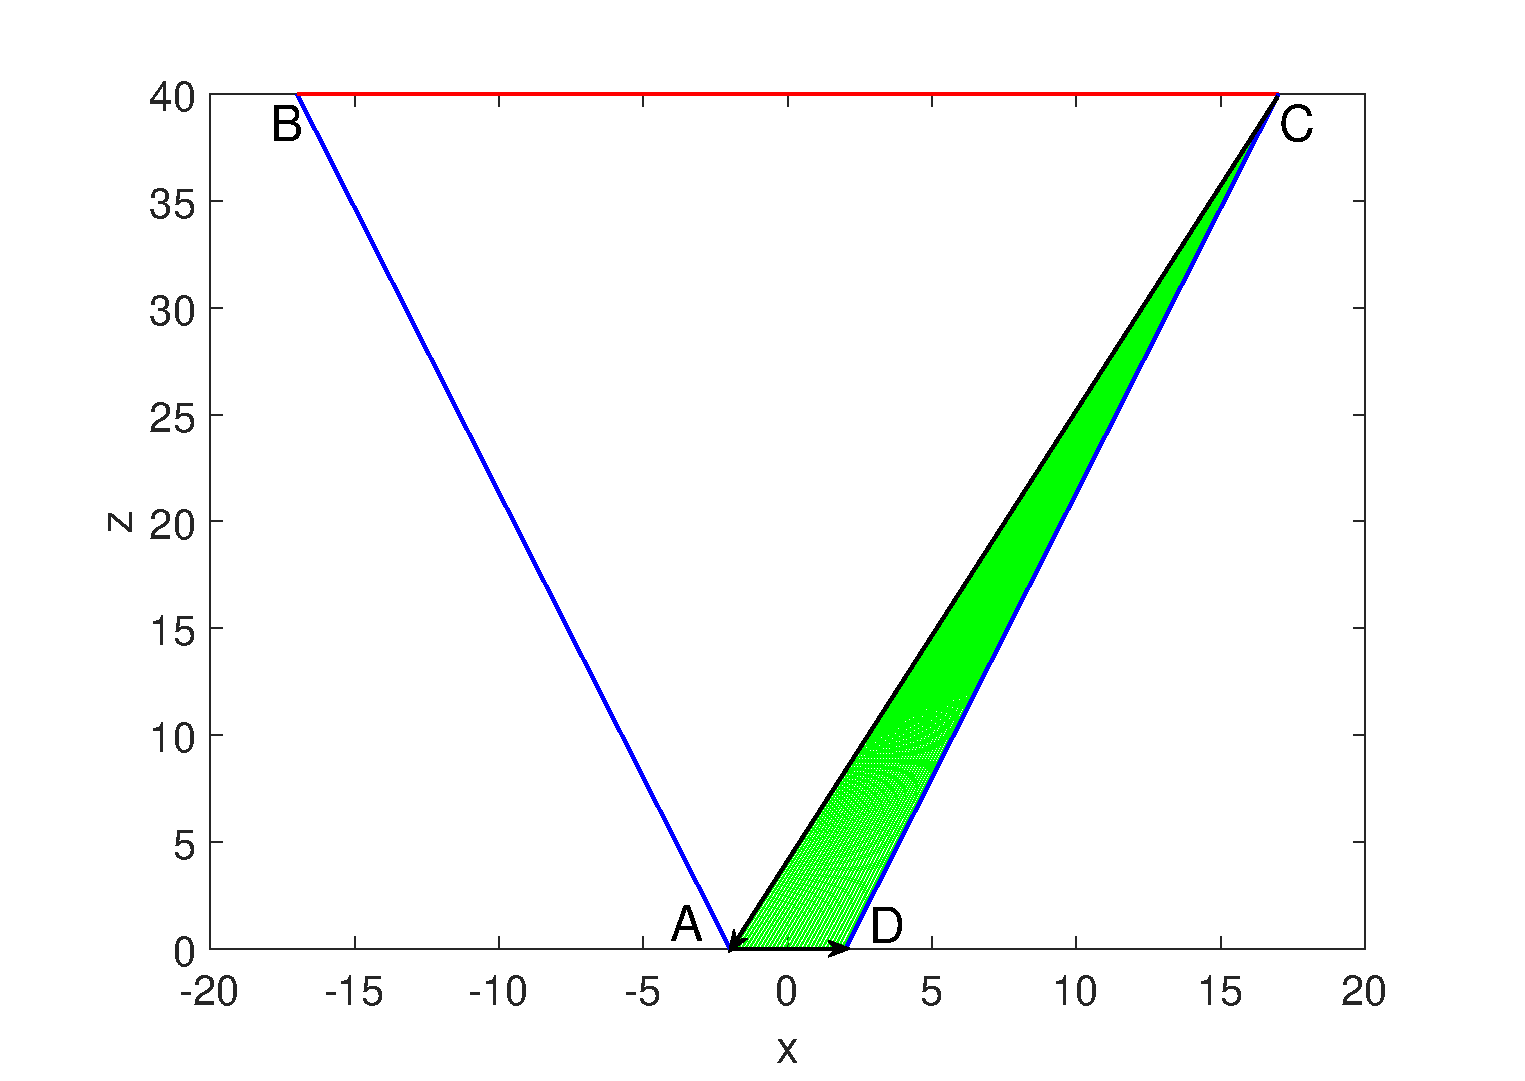
\includegraphics[width=\textwidth]{rays_cup2}
  \caption{Rays that trace out the source (line $1$) and hit the right end point of the target (line $4$).}
  \label{fig:cup2}
\end{subfigure} %
\begin{subfigure}{.48\textwidth}
  \centering
  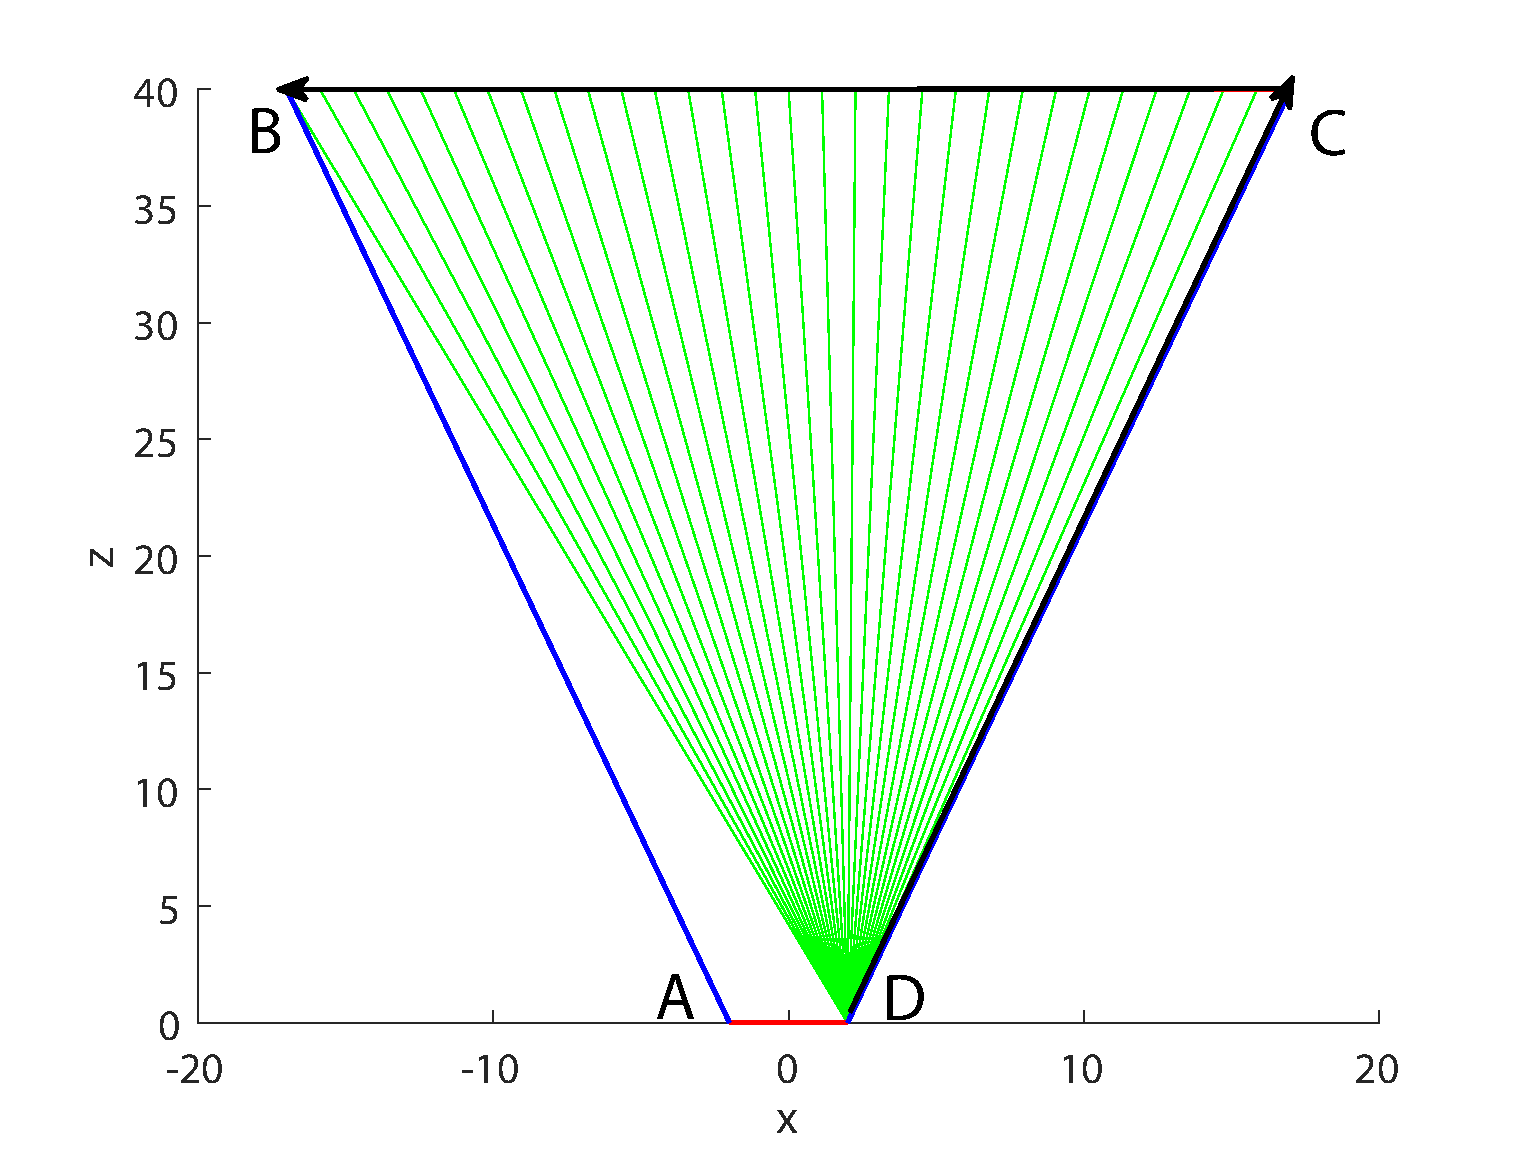
\includegraphics[width = \textwidth]{rays_cup3}
  \caption{Rays that leave the right end point of the source (line $1$) and trace out the target (line $4$).}
  \label{fig:cup3}
\end{subfigure}%
\begin{subfigure}{.48\textwidth}
  \centering
  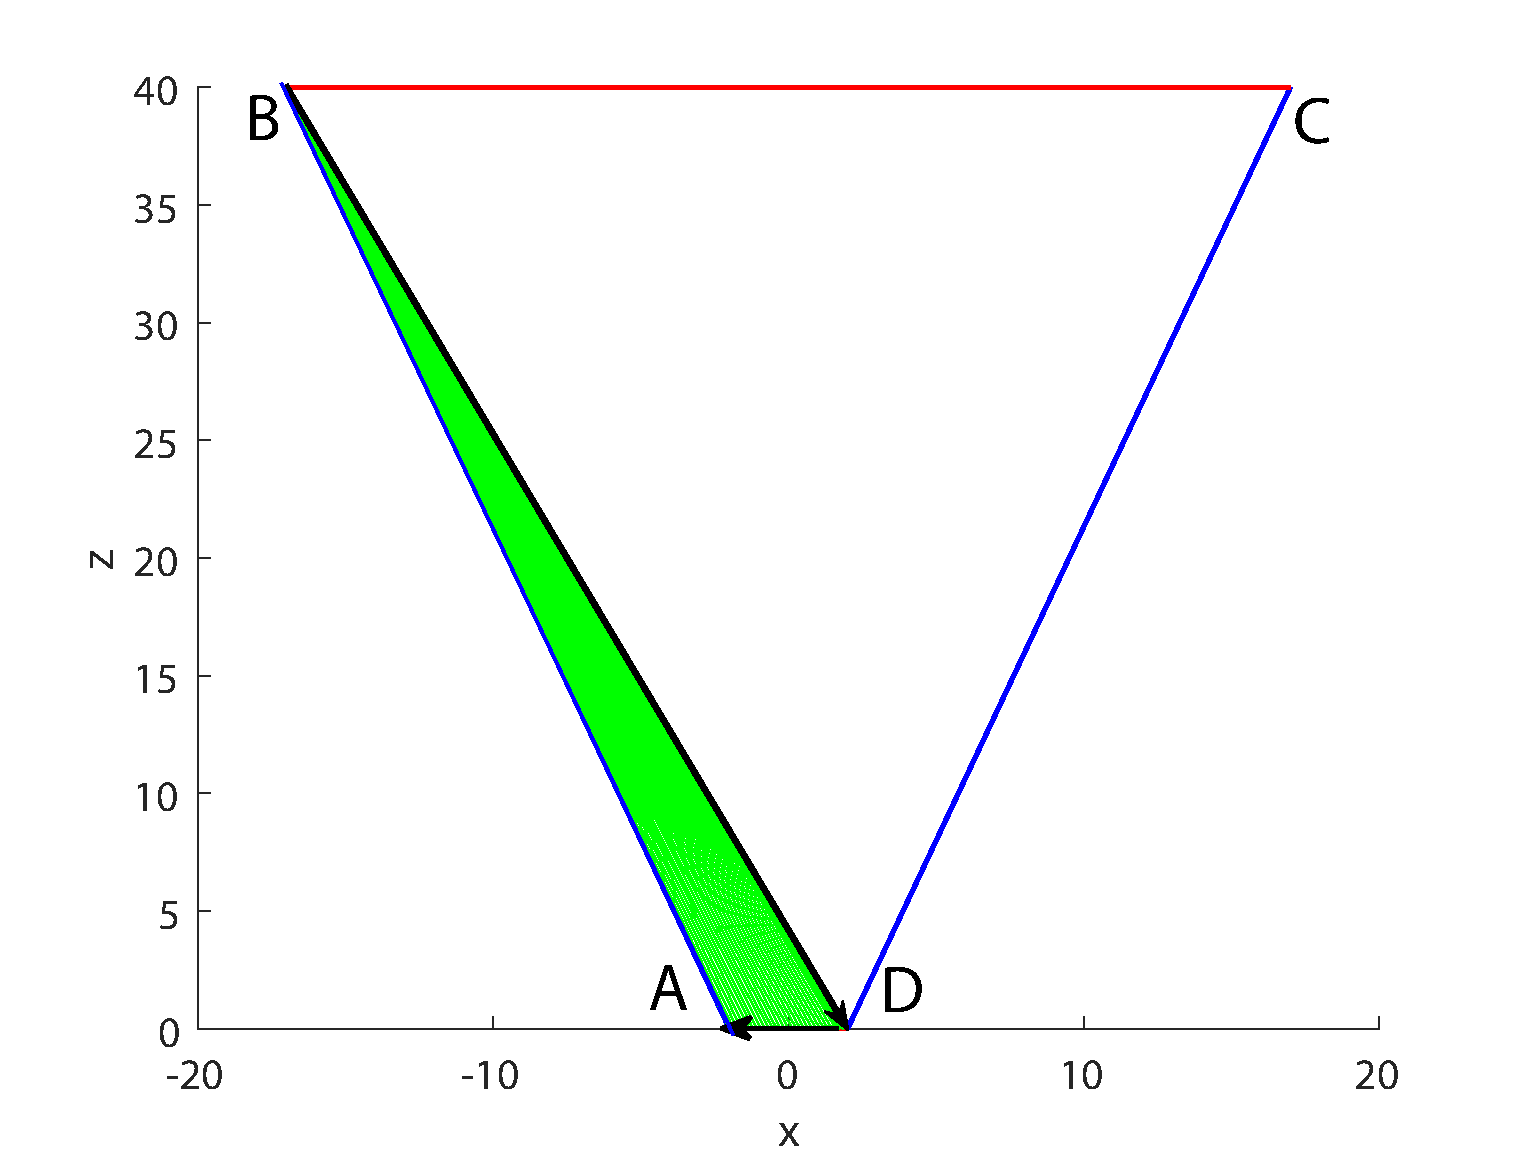
\includegraphics[width=\textwidth]{rays_cup4}
  \caption{Rays that trace out the source (line $1$) and hit the left end point of the target (line $4$).}
  \label{fig:cup4}
\end{subfigure}
\caption{Rays located on the boundaries of the regions $\partial$\set{S}{$1$,}{$4$} and $\partial$\set{T}{$4$,}{$1$}.
$A = (\variabile{x}_{1 \ell}, \variabile{z}_{1, \ell}) =(-2, 0)$ and 
$D = (\variabile{x}_{1, \textrm{r}}, \variabile{z}_{1, \textrm{r}}) = (2, 0)$ 
are the left and right corner points (or end points) of
\point{S} (line $1$), respectively.
$B =  (\variabile{x}_{4, \ell}, \variabile{z}_{4, \ell}) = (-17, 40)$ and $C =  (\variabile{x}_{4, \textrm{r}}, \variabile{z}_{4, \textrm{r}}) = (17 , 40)$, are the left and right corner points (or end points) of \point{T} (line $4$), respectively.}
\label{fig:cups}
\end{figure} \\
 The boundaries $\partial$\set{S}{$1$,}{$4$} and $\partial$\set{T}{$4$,}{$1$} are given in Figs. \ref{fig:S14} and \ref{fig:T411}, respectively.
$\partial$\setbound{S}{$1$,}{$4$}{1} and $\partial$\setbound{T}{$4$,}{$1$}{1} are obtained tracing out line $4$ from
$\variabile{q}_{4, \textrm{min}} = -\variabile{b}$ to $\variabile{q}_{4, \textrm{max}} = \variabile{b}$
 by rays leaving $\variabile{q}_{1, \textrm{min}}= -\variabile{a}$ with varying $\variabile{p}_1$, these rays are shown in Fig. \ref{fig:cup1}, and the boundary segments
 $\partial$\setbound{S}{$1$,}{$4$}{1} and $\partial$\setbound{T}{$4$,}{$1$}{1} are the orange line segments labeled with \const{c}. 
 $\partial$\setbound{S}{$1$,}{$4$}{2} and $\partial$\setbound{T}{$4$,}{$1$}{2} are given tracing out line $1$ from
 $\variabile{q}_{1, \textrm{min}}= -\variabile{a}$ to $\variabile{q}_{1, \textrm{max}}= \variabile{a}$
 with varying $\variabile{p}_1$, such that all rays hit $\variabile{q}_{4, \textrm{max}} = \variabile{b}$, these rays are shown in Fig. \ref{fig:cup2}, the boundary segments
 $\partial$\setbound{S}{$1$,}{$4$}{2} and $\partial$\setbound{T}{$4$,}{$1$}{2} are depicted in blue (lines segments labeled with \const{d}).
 Likewise, $\partial$\setbound{S}{$1$,}{$4$}{3} and $\partial$\setbound{T}{$4$,}{$1$}{3} are obtained tracing out line $4$ from
$\variabile{q}_{4, \textrm{max}}= \variabile{b}$ to $\variabile{q}_{4, \textrm{min}}= -\variabile{b}$ 
 by rays leaving $\variabile{q}_{1, \textrm{max}}=\variabile{x}_{1, \textrm{r}} = \variabile{a}$ with varying $\variabile{p}_{1}$. These rays are shown in Fig. \ref{fig:cup3}, 
 $\partial$\setbound{S}{$1$,}{$4$}{3} and $\partial$\setbound{T}{$4$,}{$1$}{3} are the red line segments labeled with \const{e}.
  Finally, $\partial$\setbound{S}{$1$,}{$4$}{4} and $\partial$\setbound{T}{$4$,}{$1$}{4} are given tracing out line $1$ from
$\variabile{q}_{1, \textrm{max}} = \variabile{a}$ to  $\variabile{q}_{1, \textrm{min}} = -\variabile{a}$ 
 with varying $\variabile{p}_{1}$, such that all rays hit $\variabile{q}_{4, \textrm{min}} = -\variabile{b}$, these rays are shown in Fig. \ref{fig:cup4}, 
 $\partial$\setbound{S}{$1$,}{$4$}{4} and $\partial$\setbound{T}{$4$,}{$1$}{4} are the green lines segments labeled with \const{f}. 
We remind that we use the notation $(\variabile{x}, \variabile{z})$ for the Cartesian coordinates system of real space, while phase space has $(\variabile{q}, \variabile{p})$ coordinates. 
It is worth noting that  $\variabile{q}_{1, \textrm{min}}=\variabile{x}_{1, \ell}$,  $\variabile{q}_{1, \textrm{max}}=\variabile{x}_{1, \textrm{r}}$,  
$\variabile{q}_{4, \textrm{min}}=\variabile{x}_{4, \ell}$ and  $\variabile{q}_{4, \textrm{max}}=\variabile{x}_{4, \textrm{r}}$.\\ \indent
 For the two-faceted cup there is an analytic expression for every line segment $\partial\mbox{\setbound{S}{\lineai,}{\lineak}{\variabile{\,j}}}$ and
 $\partial\mbox{\setbound{T}{\lineak,}{\lineai}{\variabile{\,j}}}$ in Eq. (\ref{eq:analytic_boundaries}) with $\variabile{\lineaj}\in\{1, \cdots, 4\}$.
 For instance, the rays on the boundaries $\partial\mbox{\setbound{S}{\lineai,}{\lineak}{\,1}}$ and $\partial \mbox{\setbound{T}{\lineak,}{\lineai}{\,1}}$
  are parameterized in the (\variabile{x}, \variabile{z})-plane by
 \begin{equation}
\label{extremes_rays}
\vect{r}_{\variabile{\lineai}, \variabile{\lineak}}(\variabile{t})=
\left( \begin{array}{cc}
\variabile{x}_{\variabile{\lineak}, \ell}-\variabile{x}_{\variabile{\lineai}, \ell}+t(\variabile{x}_{\variabile{\lineak}, \textrm{r}}-\variabile{x}_{\variabile{\lineak}, \ell}) \\
\variabile{z}_{\variabile{\lineak}, \ell}-\variabile{z}_{\variabile{\lineai}, \ell}+t(\variabile{z}_{\variabile{\lineak}, \textrm{r}}-\variabile{z}_{\variabile{\lineak},\ell})
\end{array} \right) \qquad \quad 0\leq t\leq 1\,.
\end{equation}
 These rays are located on a vertical line segment in \set{S}{\lineai}{} as only the $\mbox{\variabile{p}}_{\variabile{\lineai}}$-coordinate changes and on a curved line in \set{T}{\lineak}{}
  as both the target position and direction vary. The analytic expressions for $\partial \mbox{\setbound{S}{\lineai,}{\lineak}{\,1}}$ and $\partial \mbox{\setbound{T}{\lineak,}{\lineai}{\,1}}$ are
\begin{equation}
\label{S_boundary}
\partial \mbox{\setbound{S}{\lineai,}{\lineak}{1}}(\variabile{t})= \bigg\{ (\variabile{q}_{\variabile{\lineai}}, \variabile{p}_{\variabile{\lineai}}) = \Big(\variabile{q}_{\variabile{\lineai}, \textrm{min}},
|\boldsymbol{\nu}_{\variabile{\lineai}}\times \hat{\vect{r}}_{\variabile{\lineai}, \variabile{\lineak}}(\variabile{t})|
\Big), \bigg\}
\end{equation}
\begin{equation}
\label{T_boundary}
\partial\mbox{\setbound{T}{\lineak,}{\lineai}{\,1}}(\variabile{t})=\bigg\{(\variabile{q}_{\variabile{\lineak}}, \variabile{p}_{\variabile{\lineak}}) =
\Big(\variabile{q}_{\variabile{\lineak}, \textrm{max}}-\variabile{q}_{\variabile{\lineai}, \textrm{min}}+t(\variabile{q}_{\variabile{\lineak}, \textrm{max}}-\variabile{q}_{\variabile{\lineak},\textrm{min}}),
|\boldsymbol{\nu}_{\variabile{\lineak}}\times \hat{\vect{r}}_{\variabile{\lineai}, \variabile{\lineak}}(\variabile{t})|\Big) \bigg\}\,,
\end{equation}
where we have indicated with $\hat{\vect{r}}_{\variabile{\lineai}, \variabile{\lineak}}(\variabile{t})$ the normalization of the ray in Eq. ($\ref{extremes_rays}$) and,
 $ \boldsymbol{\nu}_\variabile{\lineai}$ and $\boldsymbol{\nu}_\variabile{\lineak}$ are the normalized inward normals to lines $\variabile{\lineai}$ and $\variabile{\lineak}$, respectively.
 Note that,  $\sin{\tau_\variabile{\lineai}} = |\nu_{\variabile{\lineai}}\times \hat{\vect{r}}_{\variabile{\lineai}, \variabile{\lineak}}(\variabile{t})|$ and $\sin{\tau_\variabile{\lineak}} = |\nu_{\variabile{\lineak}}\times \hat{\vect{r}}_{\variabile{\lineai}, \variabile{\lineak}}(\variabile{t})|$.
 \begin{figure}
 \begin{minipage}[]{.5\textwidth}
   \centering
   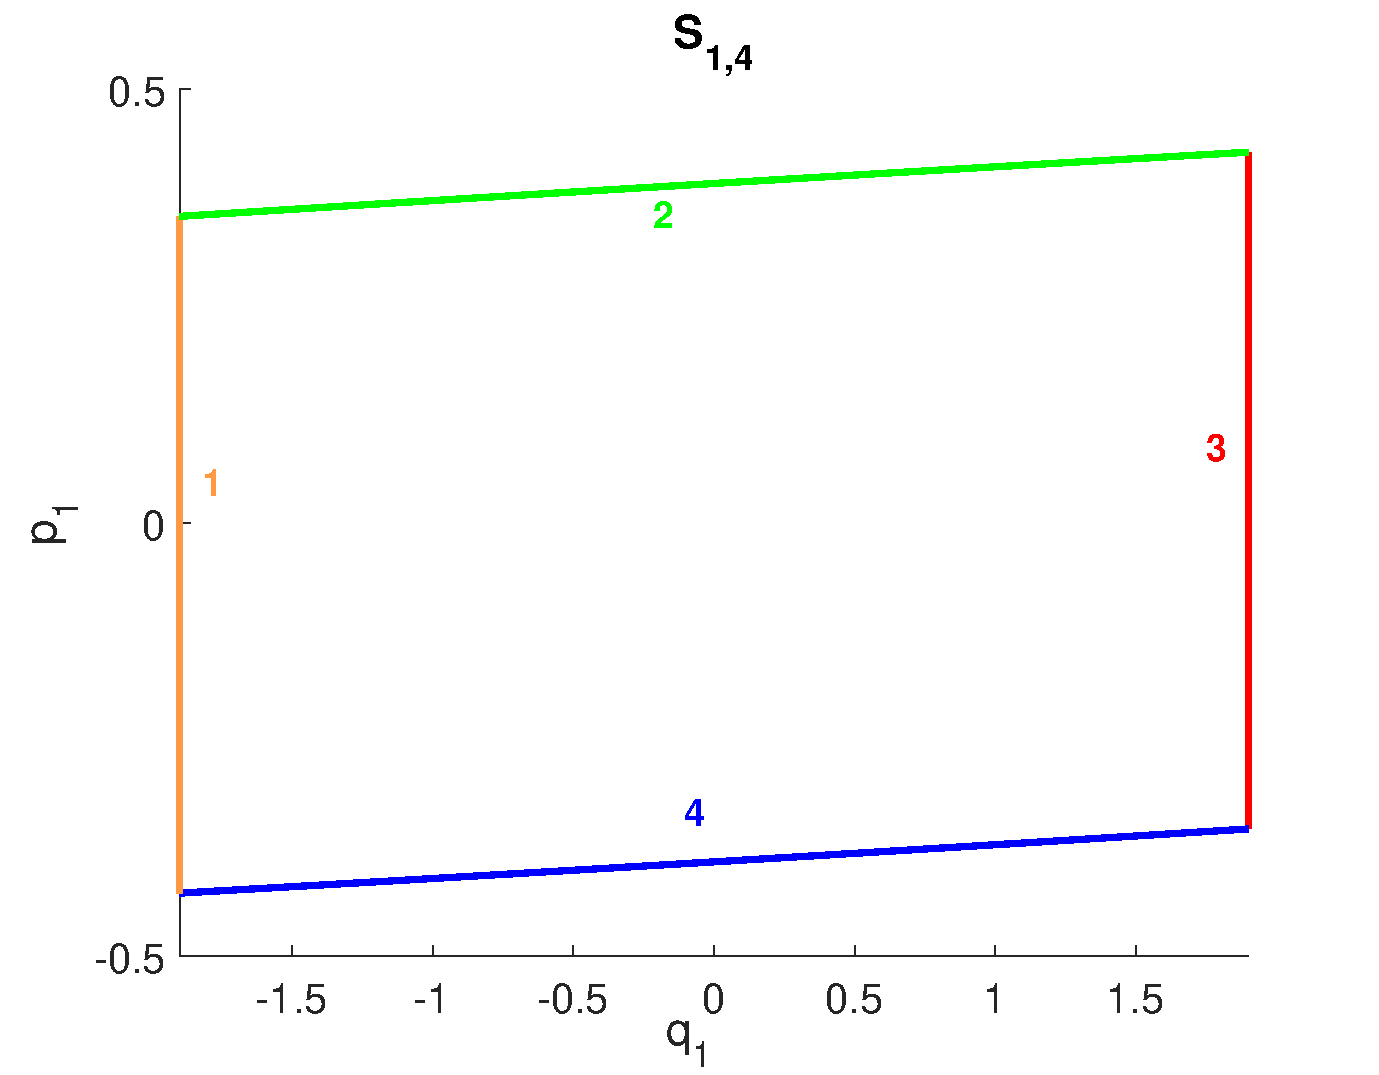
\includegraphics[width=\textwidth]{S141}
   \caption{Source phase space of line $1$.
   Boundary of the region \set{S}{$1$,}{$4$}.}
   \label{fig:S14}
 \end{minipage}
  \begin{minipage}[]{0.5\textwidth}
  \centering
   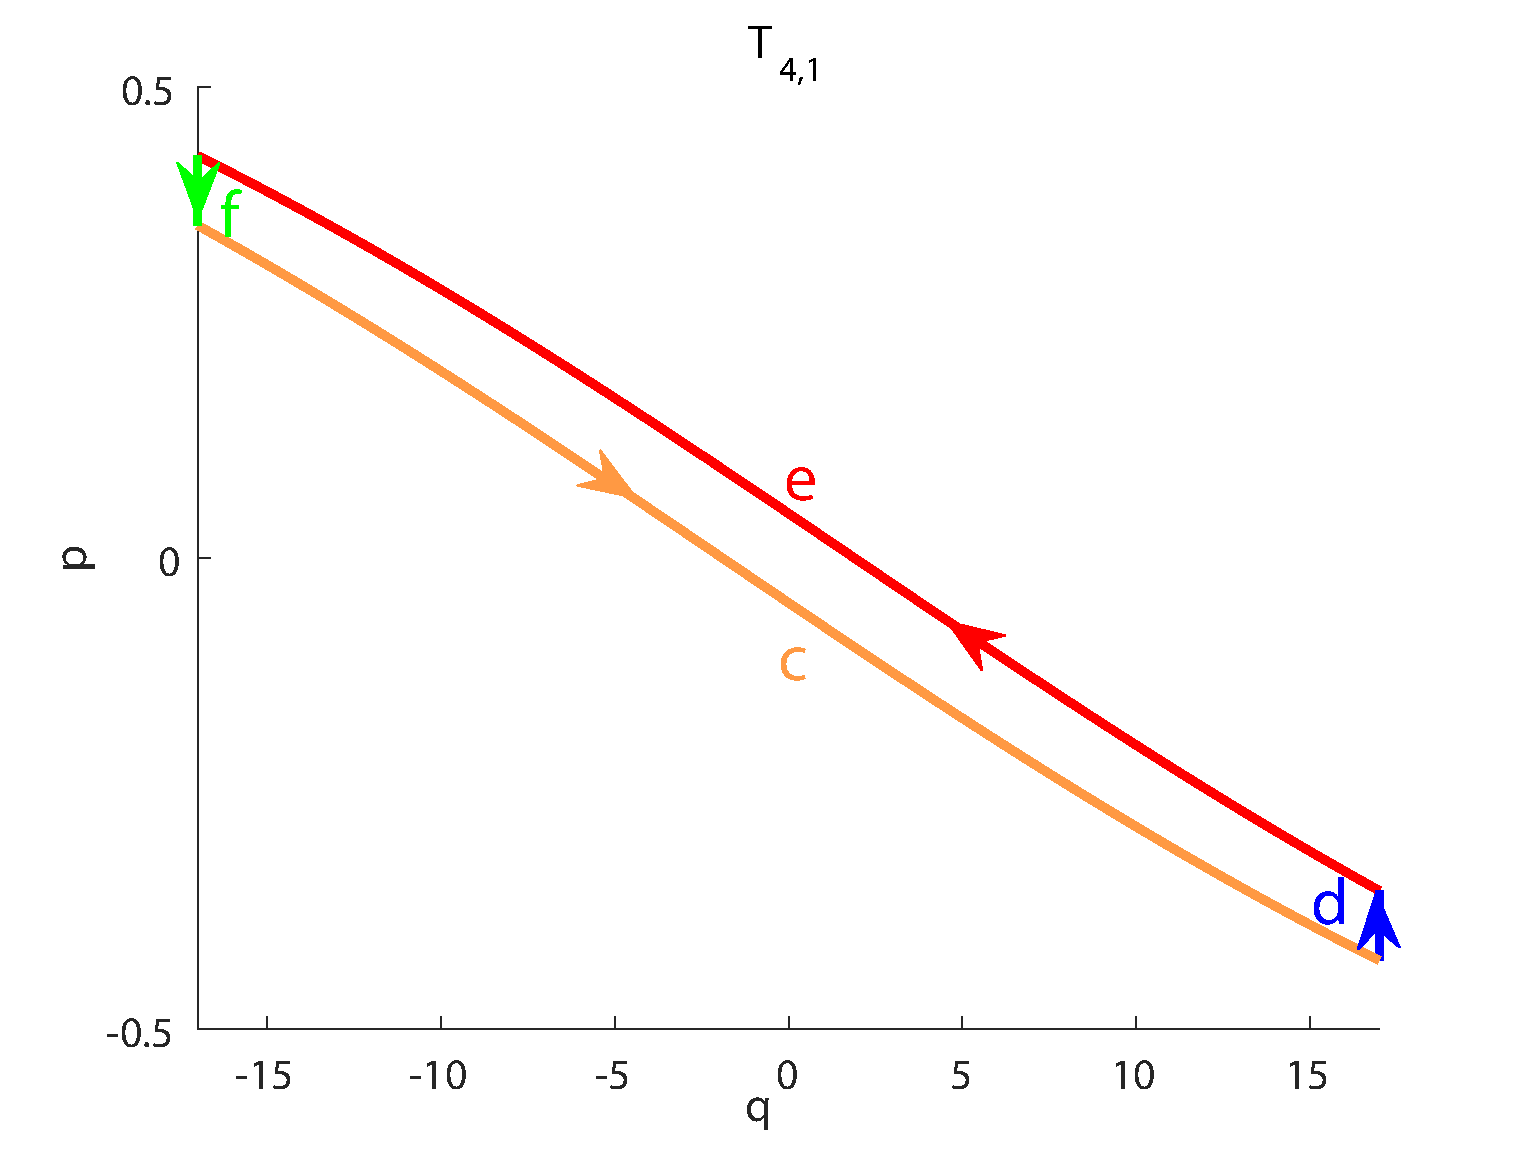
\includegraphics[width=\textwidth]{T411}
   \caption{Target phase space of line $4$.
    Boundary of the region \set{T}{$4$,}{$1$}.}
    \label{fig:T411}
 \end{minipage}
 \end{figure}
 Likewise, the boundaries $\partial$\setbound{S}{\lineai,}{\lineak}{\variabile{\lineaj}} and
 $\partial$\setbound{T}{\lineak,}{\lineai}{\variabile{\lineaj}} are calculated for every $\variabile{\lineaj}\in\{2,3,4\}$ and $\partial$\set{S}{\lineai,}{\lineak} and $\partial$\set{T}{\lineak,}{\lineai} are found using Eq. (\ref{eq:analytic_boundaries}). \\
 \begin{figure}
 \begin{minipage}[]{.43\textwidth}
   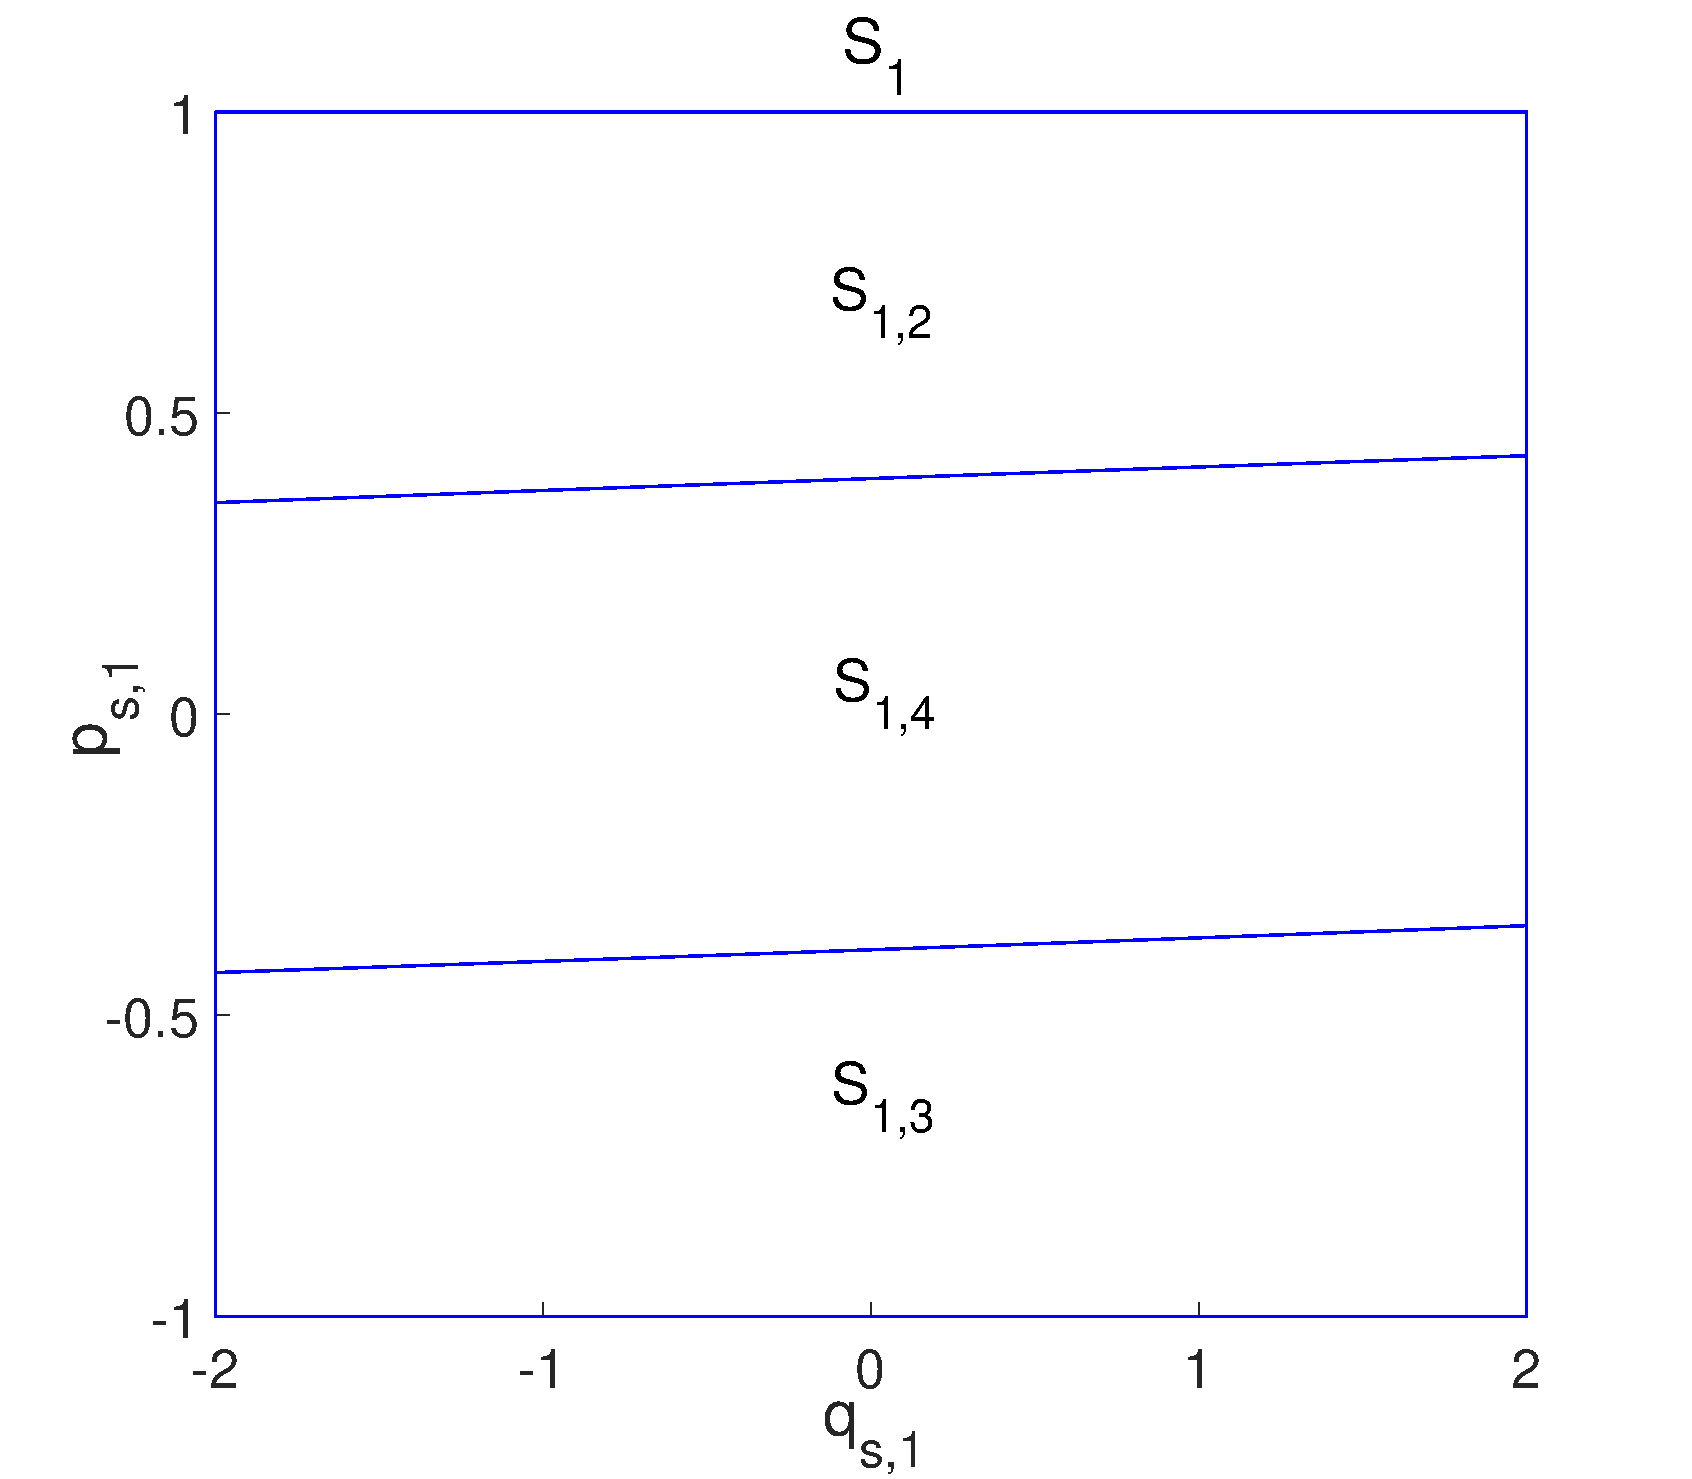
\includegraphics[width=\textwidth]{S1}
\caption{\footnotesize{The PS $\mbox{\set{S}{$1$}{}}$ of line $1$ is partitioned into regions $(\mbox{\set{S}{$1$,}{\lineaj}})_{\variabile{\lineaj} = 2,3,4}$
   formed by rays that leave line $1$ and hit line $\textit{\lineaj}$.}}
   \label{fig:S1}
 \end{minipage}
  \begin{minipage}[]{.45\textwidth}
  \centering
   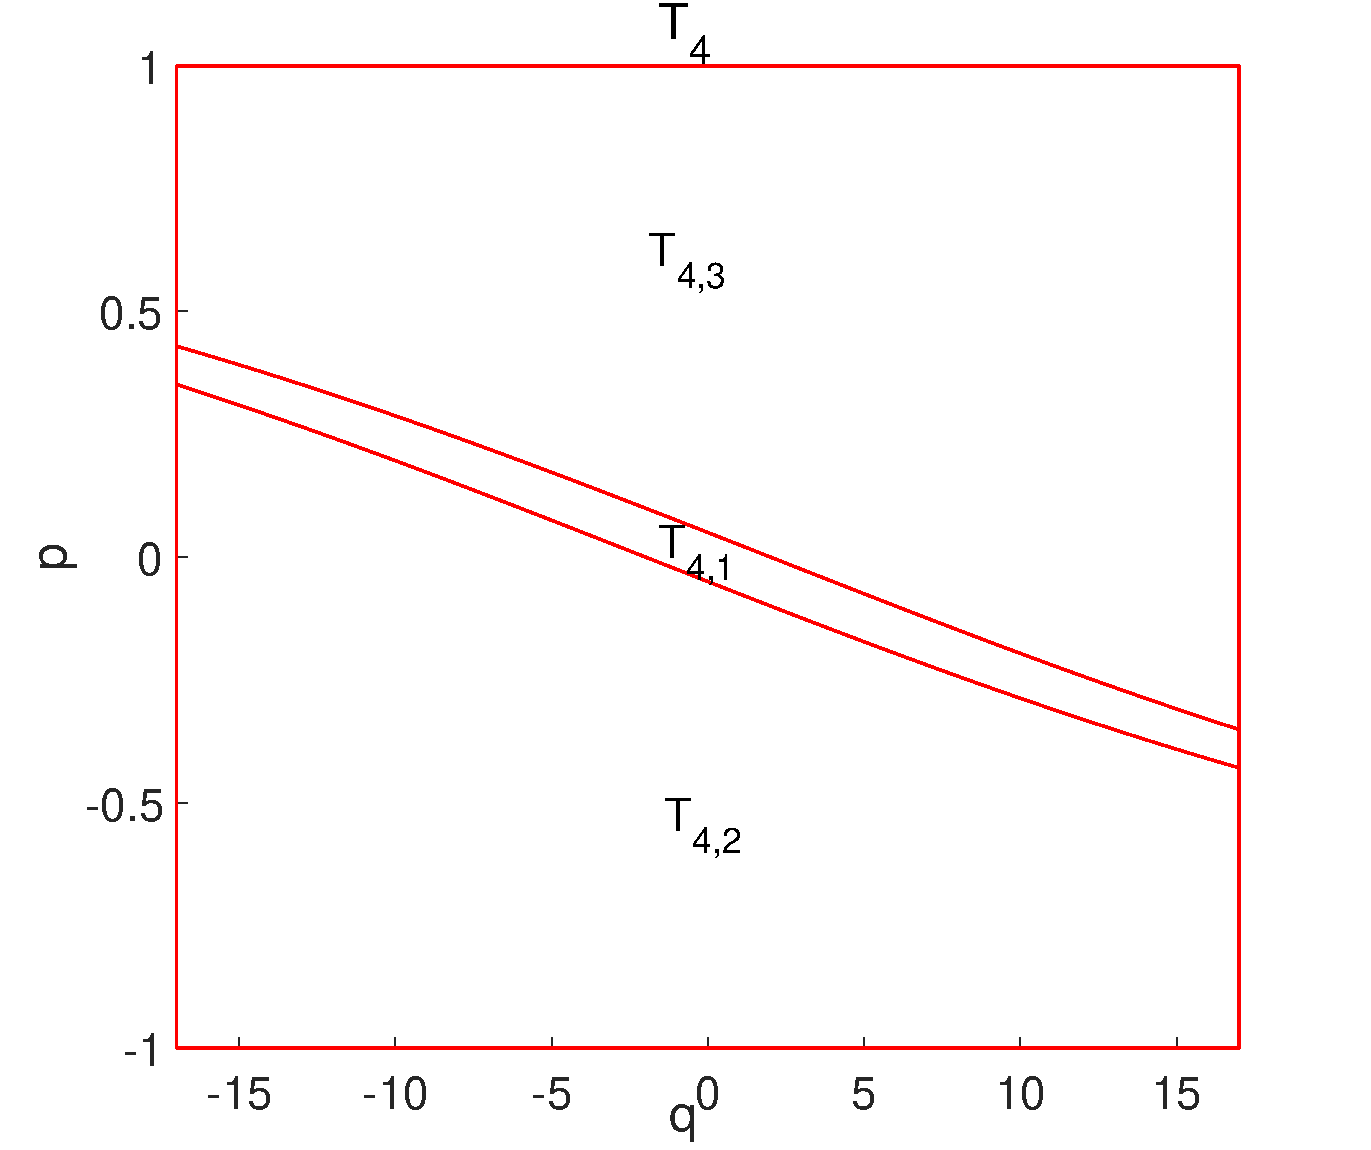
\includegraphics[width=\textwidth]{T4b}
   \caption{\footnotesize{The PS $\mbox{\set{T}{$4$}{}}$ of line $4$ is partitioned into regions $(\mbox{\set{T}{$4$,}{\lineak}})_{\variabile{\lineak} = 1,2,3}$
   formed by rays that leave line $\textit{\lineak}$ and hit line $4$.}}
   \label{fig:T4b}
 \end{minipage}
\begin{minipage}[]{.43\textwidth}
\centering
   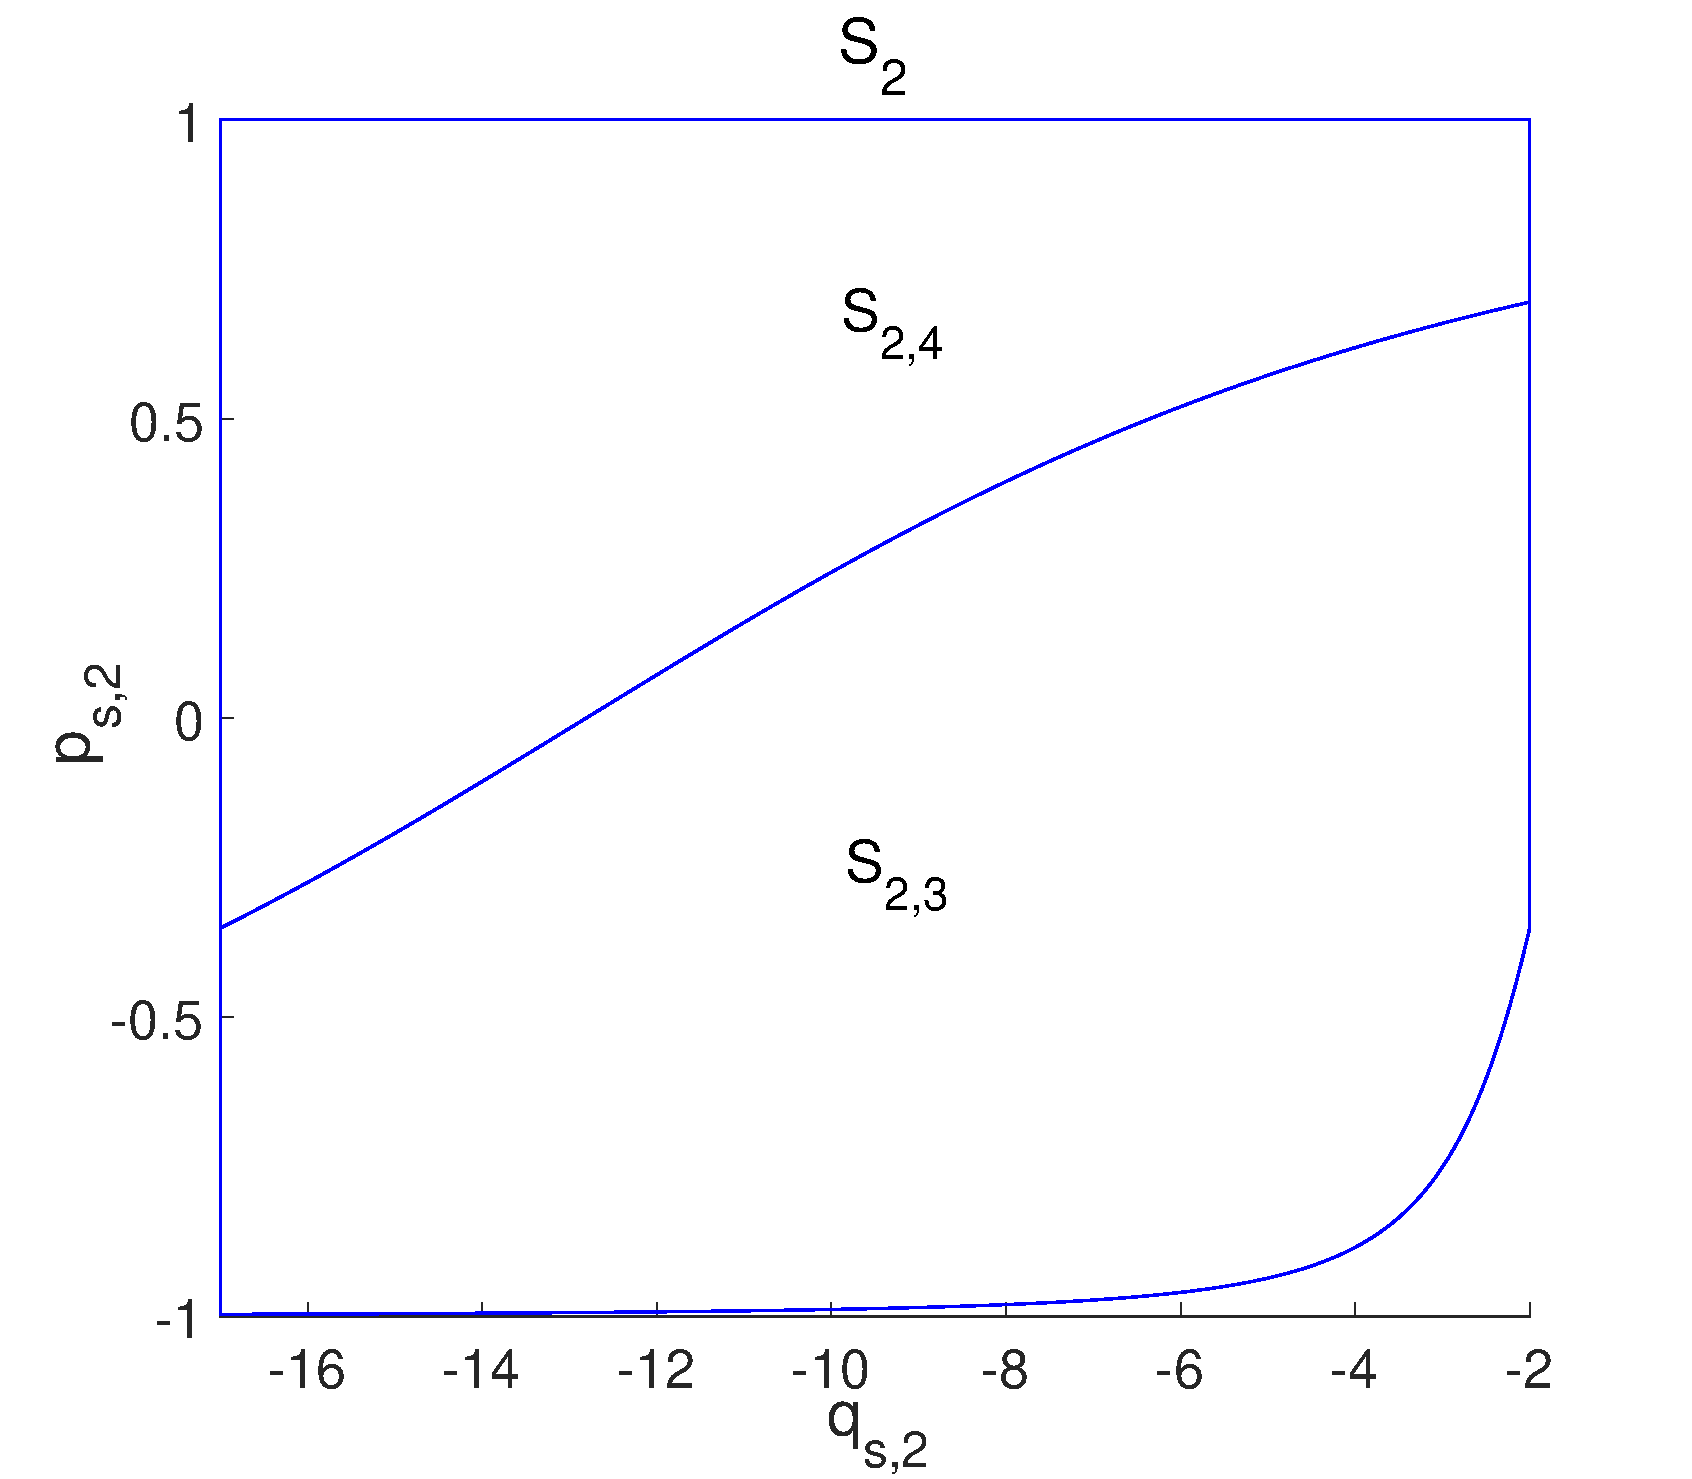
\includegraphics[width=\textwidth]{S2}
\caption{\footnotesize{The PS $\mbox{\set{S}{$2$}{}}$ of line $2$ is partitioned into regions $(\mbox{\set{S}{$2$,}{\lineaj}})_{\variabile{\lineaj} = 3,4}$
  formed by rays that leave line $2$ and hit line $\variabile{\lineaj}$.}} 
 \end{minipage}
 \begin{minipage}[]{.43\textwidth}
 \centering
   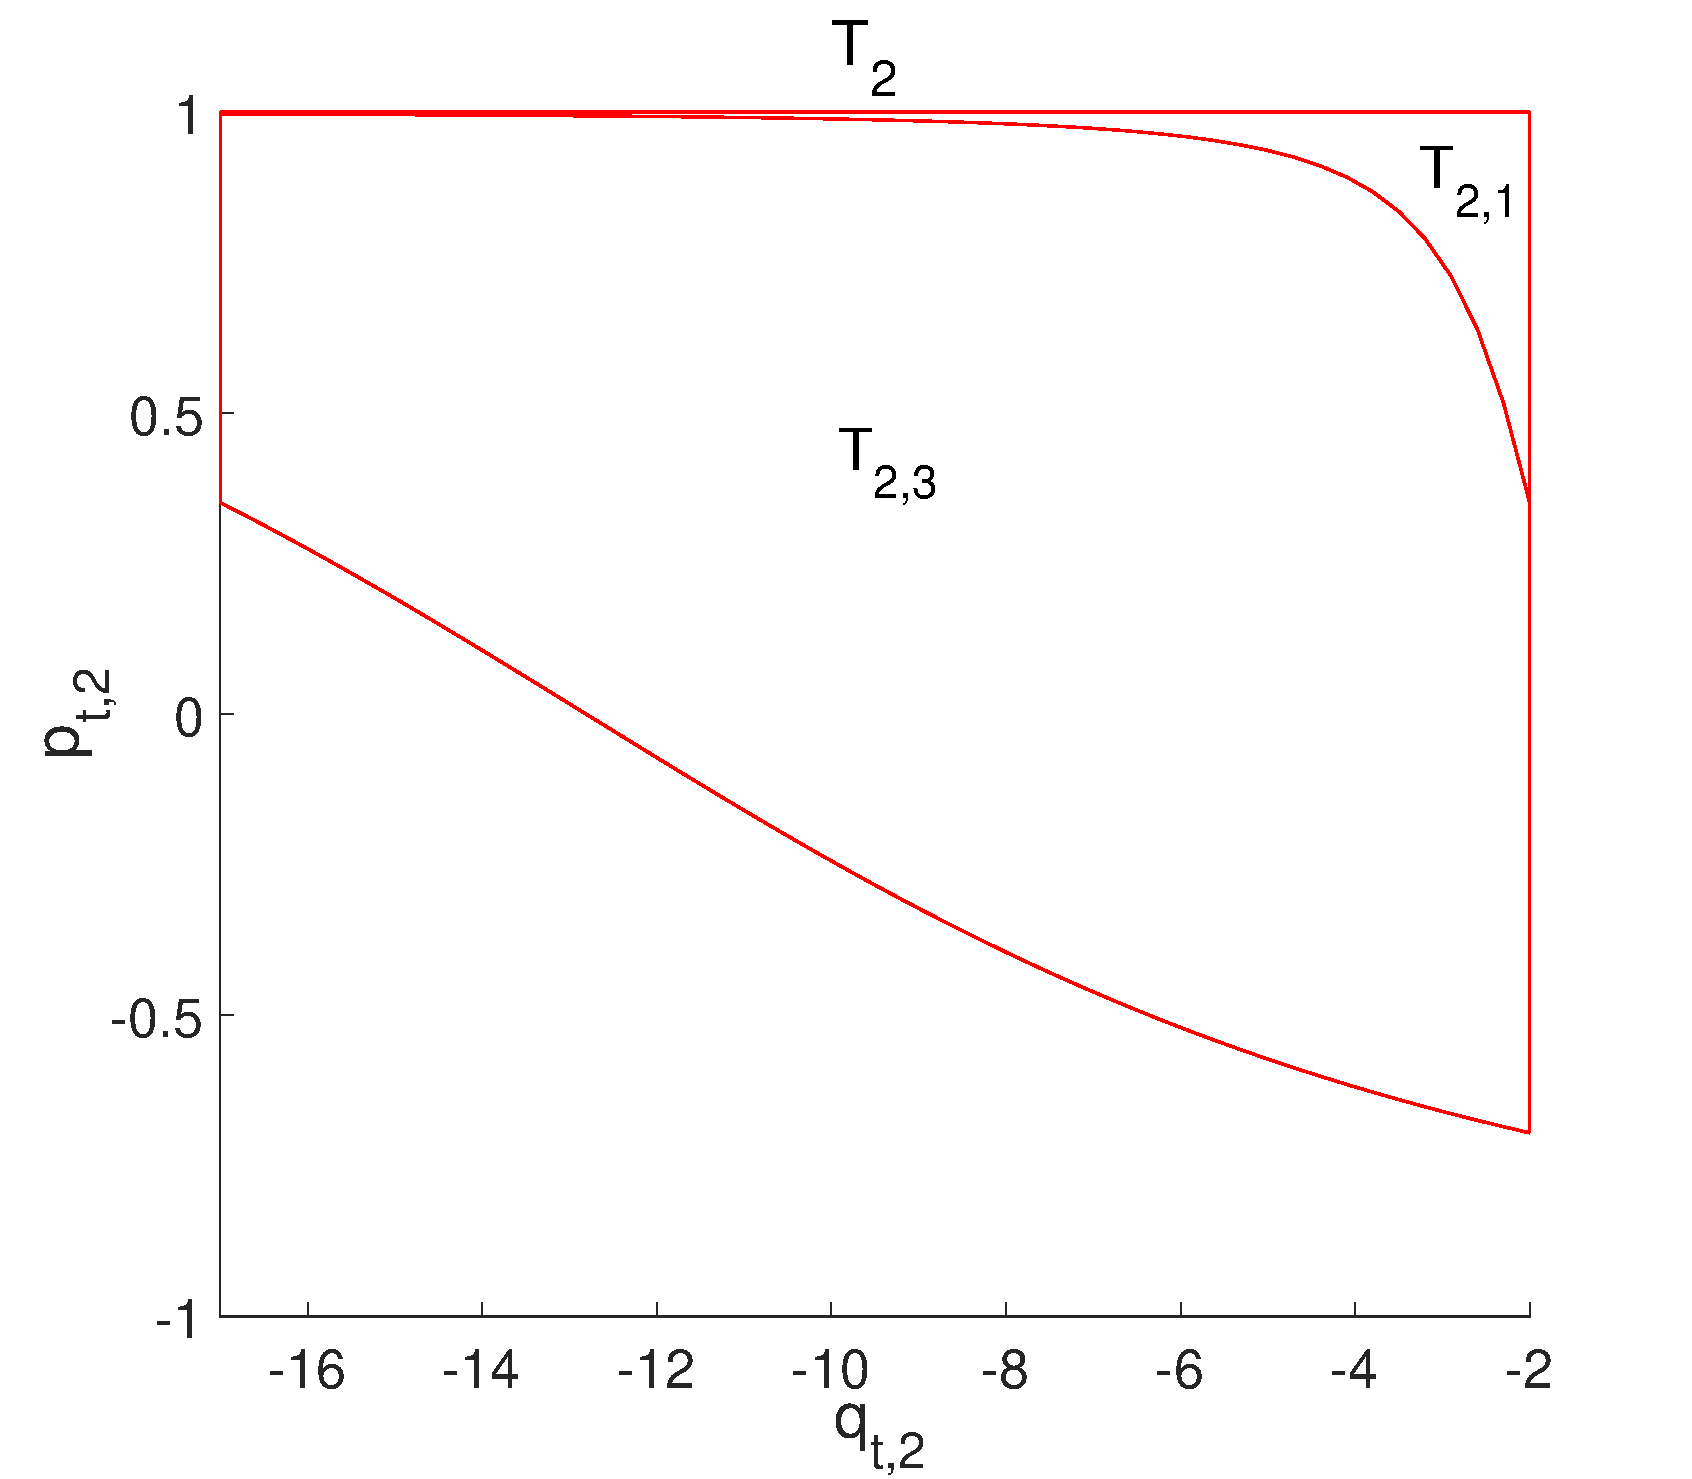
\includegraphics[width=\textwidth]{T2b}
\caption{\footnotesize{The PS $\mbox{\set{T}{$2$}{}}$ of line $2$ is partitioned into regions $(\mbox{\set{T}{$2$,}{\lineak}})_{\variabile{\lineak} = 1,3}$
formed by rays that leave line $\variabile{\lineak}$ and hit line $2$. }} 
 \end{minipage}
 \begin{minipage}[]{.43\textwidth}
 \centering
   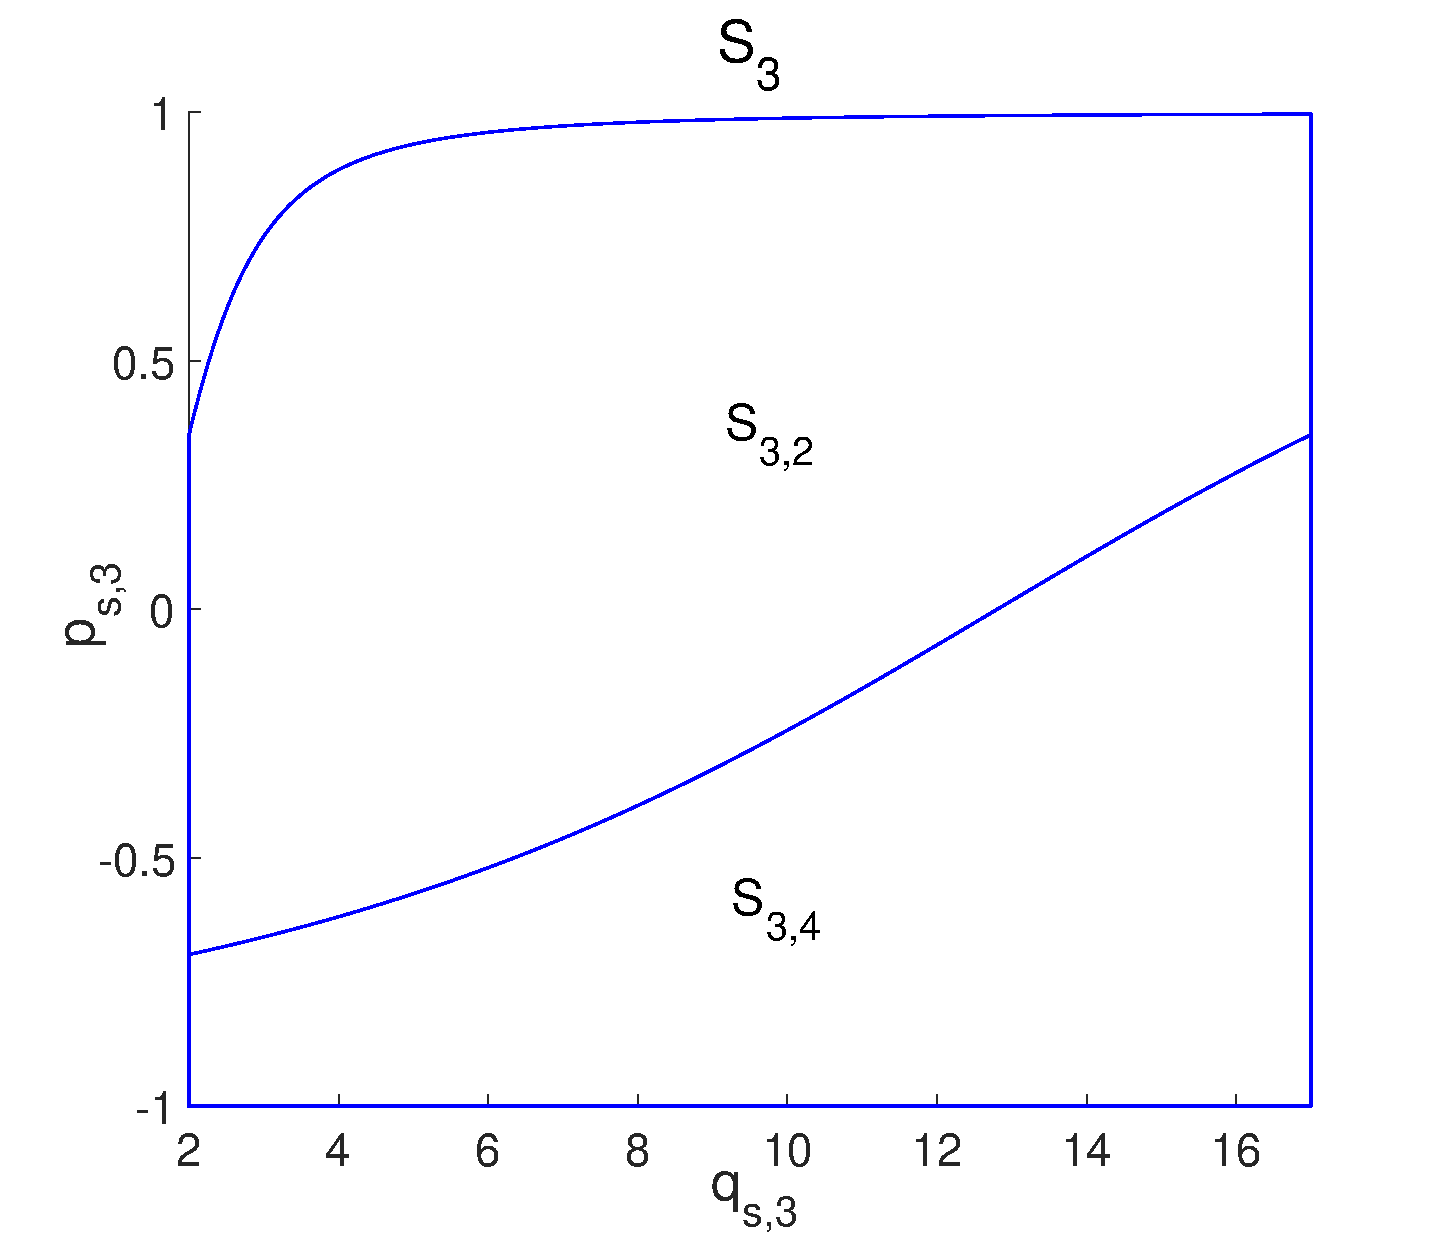
\includegraphics[width=\textwidth]{S3}
   \caption{\footnotesize{The PS $\mbox{\set{S}{$3$}{}}$ of line $3$ is partitioned into regions
   $(\mbox{\set{S}{$3$,}{\lineaj}})_{\variabile{\lineaj} = 2,4}$ formed by rays that leave line $3$ and hit line $\variabile{\lineaj}$. }} 
 \end{minipage}
 \hspace{1.7cm}
 \begin{minipage}[]{.43\textwidth}
 \centering
   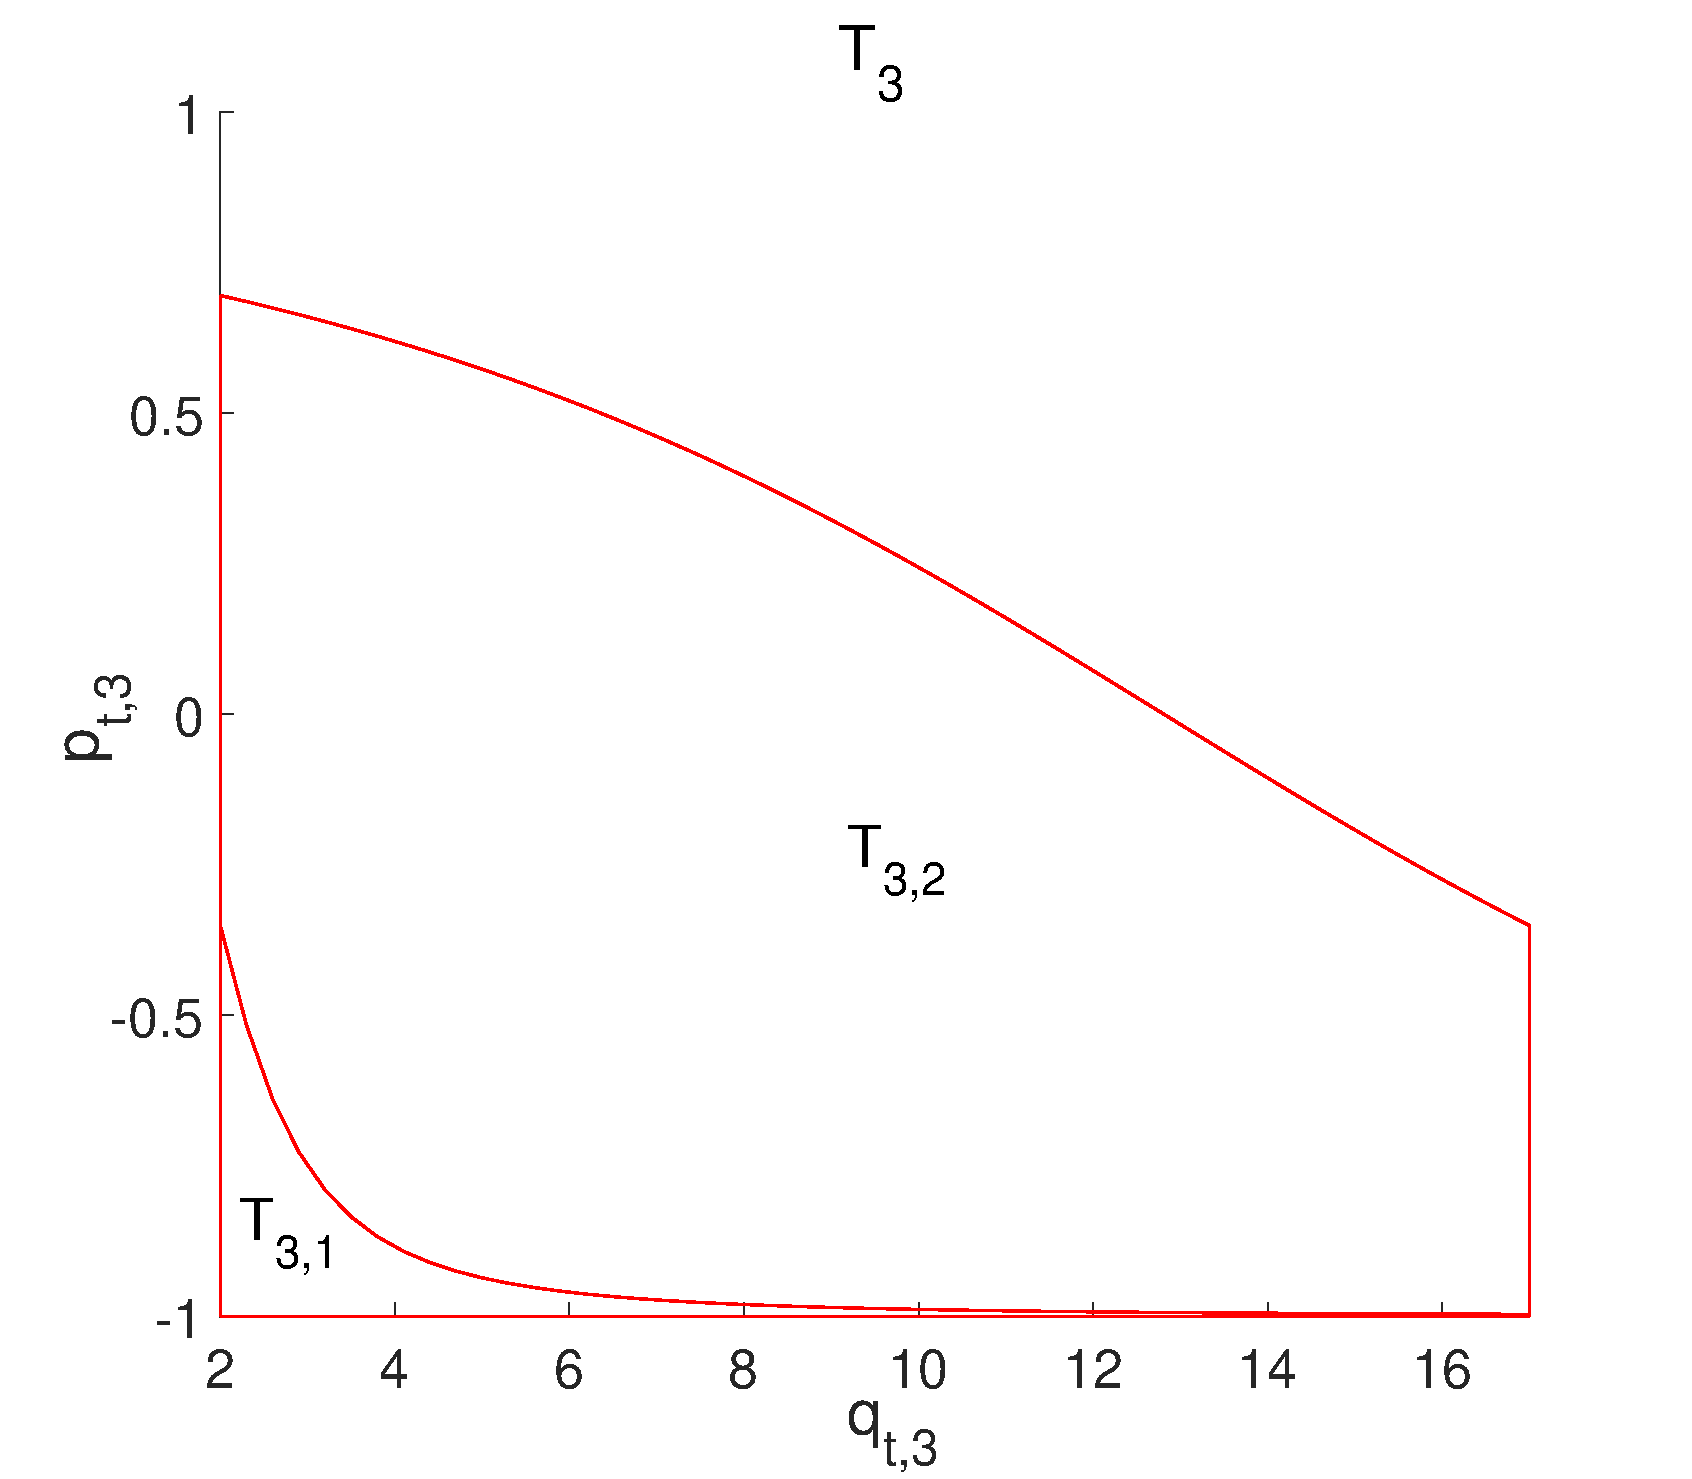
\includegraphics[width=\textwidth]{T3_b}
  \caption{\footnotesize{The PS $\mbox{\set{T}{$3$}{}}$ of line $3$ is partitioned into regions $(\mbox{\set{T}{$3$,}{\lineak}})_{\variabile{\lineak} = 1,2}$
   formed by rays that leave line $\variabile{\lineak}$ and hit line $3$.}} 
\label{fig:T3}
 \end{minipage}
\end{figure}
\indent In Figs. $\ref{fig:S1}-\ref{fig:T3}$,  $(\partial \mbox{\set{S}{\lineai,}{\lineaj}})_{\variabile{\lineai}\neq\variabile{\lineaj}=2, 3, 4}$ and $(\partial \mbox{\set{T}{\lineai,}{\lineak}})_{\variabile{\lineai}\neq\variabile{\lineak}=1, 2, 3}$ are depicted in blue and red, respectively. The source and target PS of lines $2$ and $3$ have some empty regions. 
These parts correspond to the regions formed by the rays that either go back to the source or are emitted from the target. These regions are not taken into account, see Eq. (\ref{eq:analytic_boundaries}). We observe that, because of the symmetry of the optical system, \set{S}{$3$}{} is the mirror image of \set{S}{$2$}{} after reflection in the central point 
$(\variabile{q}, \variabile{p}) = (-9.5, 0)$ and translation from $(\variabile{q}, \variabile{p})\rightarrow(\variabile{q}+19, \variabile{p})$. Likewise \set{T}{$3$}{} is the mirror image of \set{S}{$2$}{} after the same reflection and translation.
%In the next section, we show how the phase spaces are related to each other and we define the target photometric variables on \set{T}{$4$}{}.
\subsection{The structure of the algorithm}
In this section we explain how to compute the target photometric variables in PS.
In the following, to simplify the notation, we indicate the target coordinates of the rays on \set{T}{$4$}{} with (\variabile{q}, \variabile{p}) instead of $(\pos{t,}{$4$}, \dir{t,}{$4$})$.
The intensity $I$ along a given direction $\variabile{p}\in [-1,1]$ in target phase space \set{T}{$4$}{} is defined as a function of the luminance $L(\variabile{q}, \variabile{p})$:
\begin{equation}\label{I(eta)}
I_{\textrm{PS}}(\variabile{p}) = \int_{-\variabile{b}}^{\variabile{b}} L(\variabile{q},\variabile{p}) \textrm{d}\variabile{q}\,.
\end{equation}
Note that the intensity is a function of $\variabile{p}= \sin(\tau)$ instead of $\tau$.
The parts of \set{T}{$4$}{} that are illuminated by \set{S}{$1$}{} correspond to parts with positive luminance, for the other parts the luminance is equal to zero.
Assuming positive luminance on \point{S}, the following relations hold:
\begin{subequations}\label{LT4}
\begin{align}
L(\variabile{q}, \variabile{p})&>0 \qquad \quad \forall (\variabile{q}, \variabile{p})\in \mbox{\set{T}{$4$,}{$1$}},\\
L(\variabile{q}, \variabile{p})&\geq 0 \qquad\quad \forall(\variabile{q}, \variabile{p}) \in (\mbox{\set{T}{$4$,}{\lineai}})_{\lineai=2,3}.\label{third}
\end{align}
\end{subequations}
Once a ray leaves the source \point{S} it can hit the reflectors several times before hitting the target \point{T}. To relate \point{S} and \point{T}, a map \map{M}{$1$,}{$4$}: \set{S}{$1$}{}$\rightarrow$ \set{T}{$4$}{} is introduced such that $\mbox{\map{M}{$1$,}{$4$}}(\pos{s,}{$1$},\dir{s,}{$1$})=(\variabile{q},\variabile{p})$.
As  not all parts of \set{T}{$4$}{} are illuminated by the source \point{S}, the map
\map{M}{$1$,}{$4$} is not surjective.
Therefore, we need to determine the subsets of \set{T}{$4$}{} illuminated by \point{S} corresponding to the regions where the luminance is positive.
To this purpose, we consider two different kinds of maps.
The first map relates the coordinates of the source and the target PS of two \textit{different} lines, we call it the propagation map.
The second map relates the coordinates of the target and the source PS of the \textit{same} line, we call it the reflection map.
In particular, given two lines \lineai and \lineaj with \lineai$\neq$\lineaj, the propagation map \map{P}{\lineai,}{\lineaj}: \set{S}{\lineai,}{\lineaj}$\mapsto$\set{T}{\lineaj,}{\lineai} relates \set{S}{\lineai,}{\lineaj} with \set{T}{\lineaj,}{\lineai} and, it is defined as follows:
 \begin{equation}\label{Pij}
\mbox{\map{P}{\lineai,}{\lineaj}}(\pos{s,}{\lineai},\dir{s,}{\lineai})=(\pos{t,}{\lineaj},\dir{t,}{\lineaj}),
\end{equation}
where $\pos{t,}{\lineaj}$ is given by the \variabile{x}-coordinate of the intersection point between the ray and line \lineaj,
and $\dir{t,}{\lineaj}$ is computed considering the direction of the incident ray with respect to the normal of line \lineaj. 
For one single line \lineaj, the reflection map \map{R}{\lineaj,}{\lineak,}$_{h}$:~\set{T}{\lineaj,}{\lineak} $\mapsto$\set{S}{\lineaj,}{h}  relates the regions \set{T}{\lineaj,}{\lineak}$\subset$\set{T}{\lineaj}{} and
\set{S}{\lineaj,}{h}$\subset$\set{S}{\lineaj}. To simplify the notation, from now on we omit the dependence of \map{R}{\lineaj,}{\lineak,}$_{h}$ from \lineak and \variabile{h}, i.e. \map{R}{\lineaj,}{\lineak,}$_{h} = $\map{R}{\lineaj}{}.The reflection map is defined as follows:
\begin{equation}\label{Rj}
\mbox{\map{R}{\lineaj}{}}(\variabile{q}_{\textrm{t},\textit{\lineaj}},\variabile{p}_{\textrm{t},\textit{\lineaj}})=(\variabile{q}_{\textrm{s},\textit{\lineaj}},\variabile{p}_{\textrm{s},\textit{\lineaj}}),
\end{equation}
 where $\dir{t,}{\lineaj}$ changes according to the reflection law and $\pos{t,}{\lineaj}= \pos{s,}{\lineaj}$ as \map{R}{\lineaj}{} maps the target PS into the source PS of the same line \lineaj.
 Using a procedure similar to the ray transport matrices approach (see \cite{hecht1998hecht}, Chapter 6),
the map \map{M}{$1$,}{$4$} is described by the composition of mappings \map{P}{\lineai,}{\lineaj} and \map{R}{\lineaj}{} defined in Eqs.
$(\ref{Pij})$ and $(\ref{Rj})$, respectively. This composition depends on the path $\Pi$ followed by the rays where we refer to a path as the sequence of lines that
 a ray hits during its propagation from \point{S} to \point{T}. We indicate with \map{M}{$1$,}{$4$}($\Pi$)
the map \map{M}{$1$,}{$4$} restricted to path $\Pi$ and with $\mbox{\set{R}{}{}}(\Pi)\subset \mbox{\set{T}{$4$}{}}$ the regions on \set{T}{$4$}{} formed by the rays that follow path $\Pi$.
Considering all the possible paths $\Pi$ from \point{S} to \point{T}, all the regions $\mbox{\set{R}{}{}}(\Pi)$ with positive luminance on \set{T}{$4$}{} can be determined.
\\ \indent To clarify this concept, we provide the following example.
Consider a ray that is emitted from the source (line $1$), first hits the left reflector (line $2$) and finally reaches the target (line $4$).
 The path $\Pi$ followed by this ray is defined as $\Pi =(1, 2, 4)$ and
 the corresponding map $\mbox{\map{M}{$1$,}{$4$}}(\Pi):\mbox{\set{S}{$1$}{}}\mapsto \mbox{\set{R}{}{}}(\Pi)$ that describes the propagation of all rays that follow the path $\Pi$ is defined by:
\begin{equation}
\label{map_example}
\mbox{\map{M}{$1$,}{$4$}}(\Pi):\mbox{\set{S}{$1$,}{$2$}}\mapsto \mbox{\set{T}{$2$,}{$1$}}\mapsto\mbox{\set{S}{$2$,}{$4$}}\mapsto \mbox{\set{T}{$4$,}{$2$}},
\end{equation} which can be written as:
\begin{equation}
\mbox{\map{M}{$1$,}{$4$}}({\Pi}) = \mbox{\map{P}{$2$,}{$4$}}
\circ \mbox{\map{R}{$2$}{}}\circ \mbox{\map{P}{$1$,}{$2$}}\,.
\end{equation}
In general, to construct the map $\mbox{\map{M}{$1$,}{$4$}}(\Pi)$ we need to know its corresponding path $\Pi$.
To determine all possible paths $\Pi$,
instead of tracing the rays from \point{S} to \point{T}, we start considering the rays in \set{T}{$4$}{}.
In particular, along a given direction $\variabile{p}\in[-1,1]$ we consider the intersection points between the line $\variabile{p}=\mbox{const}$ and $(\partial\mbox{\set{T}{$4$,}{\lineai}})_{\lineai=1, 2, 3}$. These points are traced back to line $\lineai$ from which they are emitted and their corresponding coordinates on \set{S}{\lineai}{} and \set{T}{\lineai}{} are computed. This is done applying sequentially the maps $\mbox{\inversemap{P}{\lineai,}{$4$}}:\mbox{\set{T}{$4$,}{\lineai}}\mapsto\mbox{\set{S}{\lineai,}{$4$}}$ and $\mbox{\inversemap{R}{\lineai}{}}:\mbox{\set{S}{\lineai}{}}\mapsto\mbox{\set{T}{\lineai}{}}$.
Then the same procedure is repeated considering these new coordinates on \set{T}{\lineai}{}.
The computation stops either when the points found are emitted from the source, that is when they are located on \set{S}{$1$}{}, or when they reach again the target, that is when they are located on \set{T}{$4$}{}.
If a ray reaches \set{S}{$1$}{}, then a path $\Pi$ from \point{S} to \point{T} is found.
If a ray reaches again the target \set{T}{$4$}, then we conclude that it is not emitted by
\point{S} and therefore, it is located inside the parts of \set{T}{$4$}{} with luminance equal to zero. \\ \indent
 Finally, the inverse $\mbox{\inversemap{M}{$1$,}{$4$}}(\Pi)$ of the map \map{M}{$1$,}{$4$}$(\Pi)$ is constructed for every possible path $\Pi$.
 The map \inversemap{M}{$1$,}{$4$}$(\Pi)$ is the composition of the inverses of the propagation and the reflection maps in reverse order according to the path $\Pi$.
For instance, for path $\Pi = (1,2,4)$, \inversemap{M}{$1$,}{$4$}$(\Pi)$ is given by:
\begin{equation}
\label{inverse_map}
\mbox{\inversemap{M}{$1$,}{$4$}}({\Pi}) = \mbox{\inversemap{P}{$1$,}{$2$}}
\circ \mbox{\inversemap{R}{$2$}{}}\circ \mbox{\inversemap{P}{$2$,}{$4$}}.
\end{equation}
The steps of the procedure are shown in the graph in Fig. \ref{fig:tree} where the map in Eq. (\ref{inverse_map}) is written in red. \\
\begin{figure}
 \begin{center}
  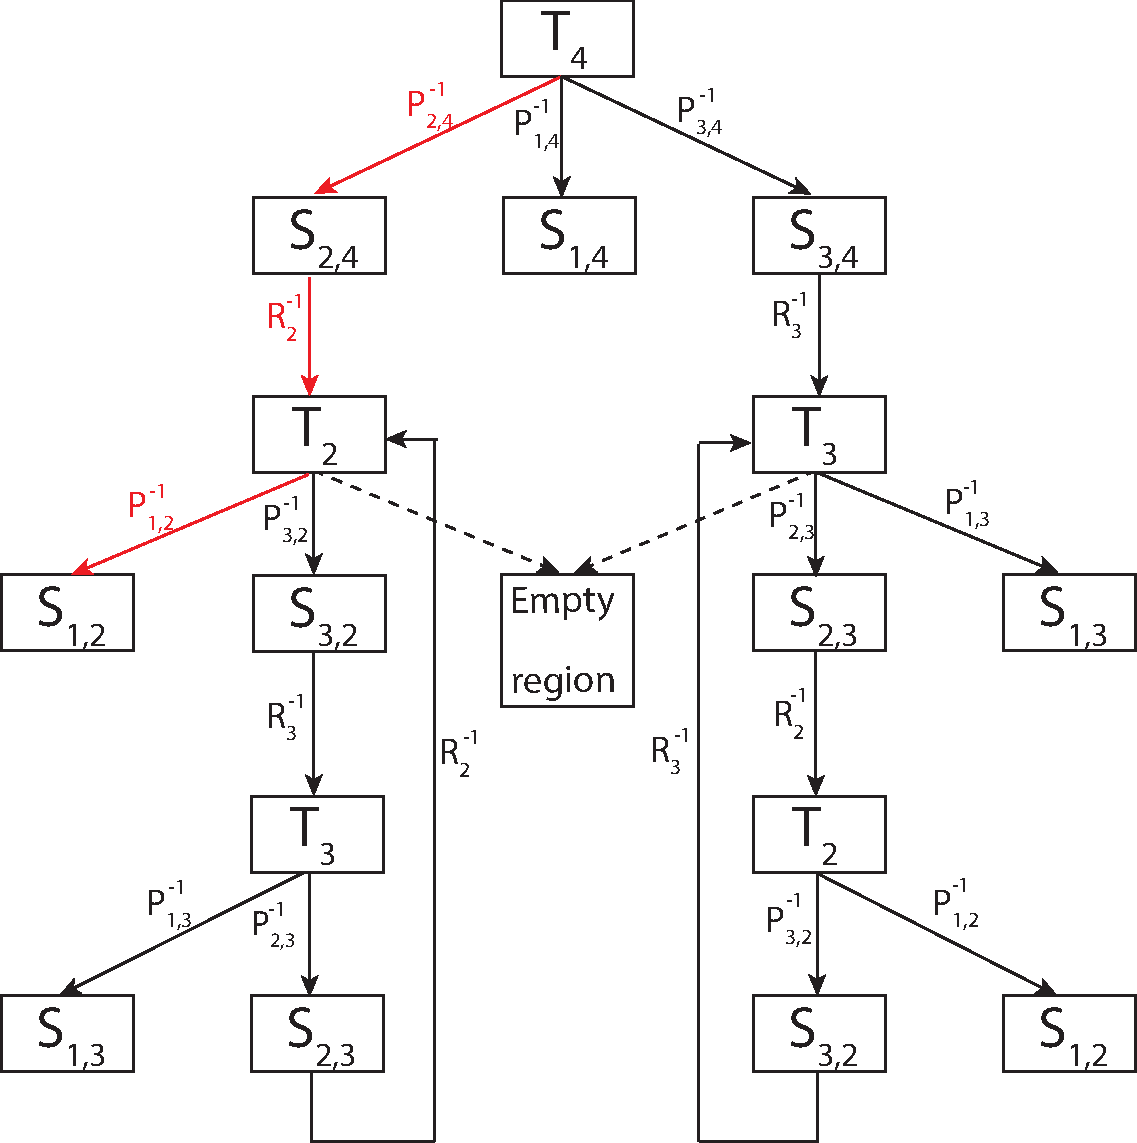
\includegraphics[width = \textwidth]{tree2}
\label{fig:tree}
  \end{center}
\caption{Tree that describes how to detect all the possible paths from \point{S} to \point{T}.}
\label{fig:tree}
\end{figure}
%\newpage
\indent Using the procedure explained above, given a ray with coordinates
$(\variabile{q}, \variabile{p})\in \mbox{\set{T}{$4$}{}}$ we can establish whether it is located inside one of the regions $\mbox{\set{R}{}{}}(\Pi)$ with positive luminance or not.
In case the ray is inside a region $\mbox{\set{R}{}{}}(\Pi)$,
its corresponding coordinates $(\pos{s,}{$1$},\dir{s,}{$1$})\in \mbox{\set{S}{$1$}{}}$ are obtained using $\mbox{\inversemap{M}{$1$,}{$4$}}(\Pi)$, where $\Pi$ is the path followed by this ray. Eq. ($\ref{LT4}$) becomes:
\begin{subequations}\label{LT}
\begin{align}
L(\variabile{q}, \variabile{p})&>0 \qquad \quad \forall (\variabile{q}, \variabile{p})\in \mbox{\set{R}{}{}}(\Pi),\\
L(\variabile{q}, \variabile{p})&= 0 \qquad \quad \mbox{otherwise},\label{third}
\end{align}
\end{subequations}
for some path $\Pi$ connecting \point{S}{}{} and \point{T}{}{}.
Assuming a Lambertian source and employing conservation of luminance along a ray (see \cite{chaves2015introduction}, Chapter 16), we have that $L$
is a positive constant inside \set{R}{}{}($\Pi$) and it has no contribution on the other parts of \set{T}{$4$}{}.
Indicating with $\variabile{q}^\textrm{\,min}(\Pi,\variabile{p})$ and $\variabile{q}^\textrm{\,max}(\Pi,\variabile{p})$ the minimum and maximum position coordinates of the intersection points between the boundaries $ \partial$\set{R}{}{}($\Pi$) and line $\variabile{p}= \mbox{const}$,
Eq. (\ref{I(eta)}) reduces to:
\begin{equation}\label{eta2}
I_{PS}(\variabile{p}) = \sum_{\Pi}\int_{\variabile{q}^\textrm{\,min}(\Pi, \variabile{p})}^{\variabile{q}^\textrm{\,max}(\Pi,\variabile{p})}L(\variabile{q}, \variabile{p})\textrm{d}\variabile{q} =
\sum_{\Pi}\big (\variabile{q}^\textrm{max}(\Pi,\variabile{p})-\variabile{q}^\textrm{\,min}(\Pi,\variabile{p})\big )\,,
\end{equation}
where the sum is over all the possible paths and the second equation holds as we assume $L=1$ in \set{R}{}{}($\Pi$). 
Note that for a given ray with corresponding coordinates $(\pos{}{}, \dir{}{})$ on \set{T}{$4$}{}, only one path is possible as we are assuming that all lines are reflective lines.
Because of this, the regions \set{R}{}{}($\Pi$) do not overlap each other, i.e. 
\begin{equation}
\bigcap_{\Pi}\mbox{\set{R}{}{}}(\Pi)= \emptyset,
\end{equation}
where the intersection is over all the possible paths. 
In the next paragraph the details of the procedure to compute the coordinates $\variabile{q}^\textrm{\,min}(\Pi, \variabile{p})$ and $\variabile{q}^\textrm{\,max}(\Pi, \variabile{p})$
are explained. 
\section{Results for the two-faceted cup}
\section{Results for the multi-faceted cup}
\section{Discussions}